\documentclass[a4paper,12pt]{article}

\usepackage[utf8]{inputenc}
\usepackage{amsmath, amssymb}
\usepackage{graphicx}
\usepackage{float}
\usepackage{caption}
\usepackage{geometry}
\usepackage{hyperref}
\usepackage{enumitem}
\usepackage{textcomp}
\usepackage{xcolor}

\geometry{a4paper, margin=1in}

\title{Laborbericht: Messtechnik und Fehlerrechnung}
\author{Helen Klos \\Matrikelnummer: 2222449 \\ \\Sandro Fahrion \\Matrikelnummer: 6684592}
\date{29.-30.10.2024}

\begin{document}
\hyphenpenalty=1000
\exhyphenpenalty=1000
\sloppy
\setlength{\emergencystretch}{5pt}
\maketitle

\begin{figure}[H]
    \centering
    \includegraphics[width=1.0\textwidth]{../Quellen/Labor2/Titelbild2.jpg}
\end{figure}
\newpage
\tableofcontents
\newpage

\section*{Einführung und Überblick}
\addcontentsline{toc}{section}{Einführung und Überblick}
Die moderne Messtechnik bildet die Grundlage zahlreicher technischer sowie naturwissenschaftlicher Erkenntnisse. Dabei ist jedoch zu berücksichtigen, dass Messergebnisse nie vollständig fehlerfrei sind. Die Ursachen für Messfehler und -ungenauigkeiten sind vielfältig. Diese können beispielsweise in einer fehlenden Kalibrierung, in der Linearität und Stabilität der verwendeten Messinstrumente oder in einer mangelnden Qualität des Messobjekts liegen. Darüber hinaus kann auch die messende Person selbst, als Ursache für den Messfehler, in Betracht gezogen werden, welche, zum Beispiel aufgrund einer möglichen Sehschwäche oder eines ungünstigen Blickwinkels, die Messwerte ungenau abliest. Auch unangepasste oder unvollkommene Messmethoden können zu einer Verfälschung der Messung führen.\\\\
Die genannten Ursachen können zu drei verschiedenen Fehlerarten führen: grobe, statistische und systematische Fehler.\\
Um die Qualität und die Aussagekraft von Messergebnissen beurteilen zu können, gibt es die Fehlerrechnung. Mit ihrer Hilfe kann der Rahmen bestimmt werden, in dem die Messung zuverlässig ist.\\\\
\noindent In diesem Laborbericht werden verschiedene Experimente beschrieben, die sich mit der Genauigkeit und Funktionsweise unterschiedlicher Bauteile und Messmethoden beschäftigen. Ziel ist es, die verschiedenen Fehlerarten systematisch zu untersuchen und deren Einfluss auf die Messergebnisse zu analysieren. Dazu werden Fehlerrechnungen durchgeführt, um die Unsicherheiten der Messungen zu quantifizieren und mögliche Ursachen für Abweichungen zu identifizieren.


\newpage

\section{Versuch 1: Kapazitätsmessung eines unbekannten Kondensators (Black Box)}

\subsection{Zielsetzung}
Für den ersten Versuch war eine Black-Box gegeben. Diese beinhaltete einen Kondensator, mit einer unbekannten Größe zwischen $1 nF$ und $10 nF$. Das Ziel des ersten Versuchs bestand darin, die Kapazität dieses unbekannten Kondesators zu bestimmen. 

\subsection{Bauteile und Messgeräte}
\subsubsection*{Messgeräte}
\begin{itemize}
\item Teledyne Technologies Funktionsgenerator T3AFG80 80 MHz
\item Keysight Oszilloskop (DSOX1102A)
\item Fluke 87 V True RMS Multimeter
\item Oszilloskop BNC Tastkopf mit Messklemme
\item Steckkabel (mehrere)
\item Tru Components Steckbrett
\item Bananenkabel (schwarz und rot)
\item Sicherheits-Klemmprüfspitze (2 Stück)
\end{itemize}

\subsubsection*{Bauteile}
\begin{itemize}
\item Black-Box (Nr. 18-30)
\item Widerstand Nominalwert 4,7 k$\Omega$, Toleranz 5~\%
\end{itemize}




\subsection{Messkonzept}
Zu Beginn wurde die Formel der Ladekurve \( u\textsubscript{c} = U (1 -e ^{-\frac{t}{RC}}) \) und der Entladekurve  \( u\textsubscript{c} = Ue ^{-\frac{t}{RC}}) \) grafisch am Computer dargestellt (siehe Figure 1). 

\begin{figure}[H]
    \centering
    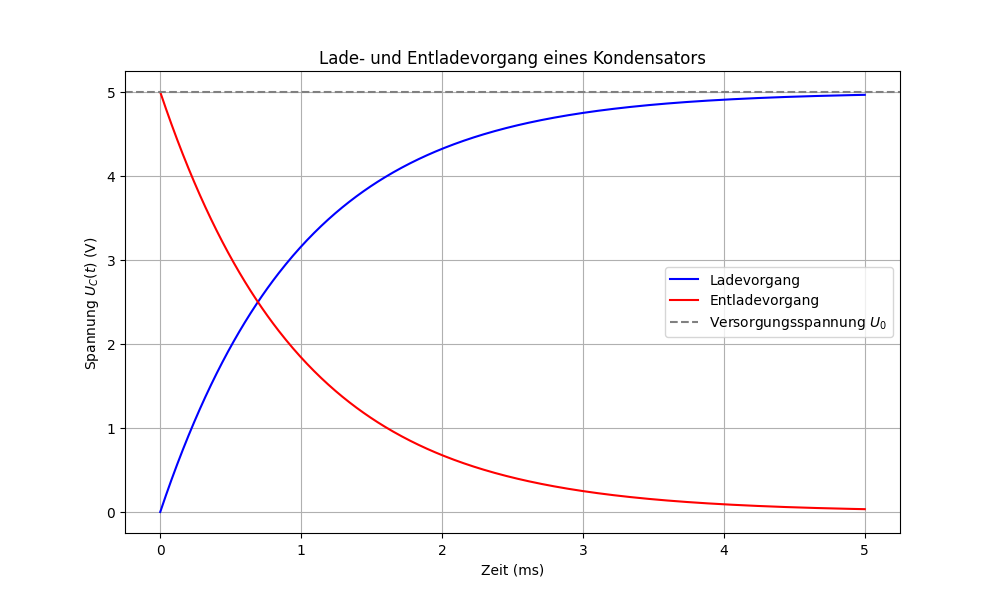
\includegraphics[width=0.9\textwidth]{../Quellen/Labor2/Lade-EntladefunktionSkizze.png}
\caption{Ladekurve (blau) und Entladekurve (rot) eines Kondensators}
\end{figure}

\noindent Diese sollte in den folgenden Schritten mit dem Oszilloskop sichtbar gemacht werden. Hierzu wurde sich zunächst überlegt, wie der Funktionsgenerator einzustellen ist. Diese Einstellungen sind Table 1 zu entnehmen. Für die verwendete Frequenz muss dabei gelten, dass die Periode \(T~=~\frac{1}{f}\) wesentlich größer ist als die Zeitkonstante, um die vollständige Ladung und Entladung sichtbar zu machen.

\begin{table}[H]
	\centering
	\begin{tabular}{|c|c|c|c|}
		\hline
		\textbf{Frequenz in Hz} & \textbf{Signalform} & \textbf{Amplitude in V\textsubscript{pp}} & \textbf{Offset in V\textsubscript{dc}}\\
		\hline
		500 & Rechtecksignal & 5 & 2.5\\
		\hline
	\end{tabular}
	\caption{Einstellungen des Funktionsgenerators}
\end{table}

\noindent Nachem der Funktionsgenerator korrekt eingestellt war, wurde die Schaltung  für die Messungen aufgebaut. Dabei wurde sich an der in Figure 2 dargestellten Skizze orientiert. Der, in der Skizze dargestellte, 50~$\Omega$ Widerstand ist der Innenwiderstand des Funktionsgenerators. Dieser muss bei späteren Rechnungen berücksichtigt werden.\\

\begin{figure}[H]
    \centering
    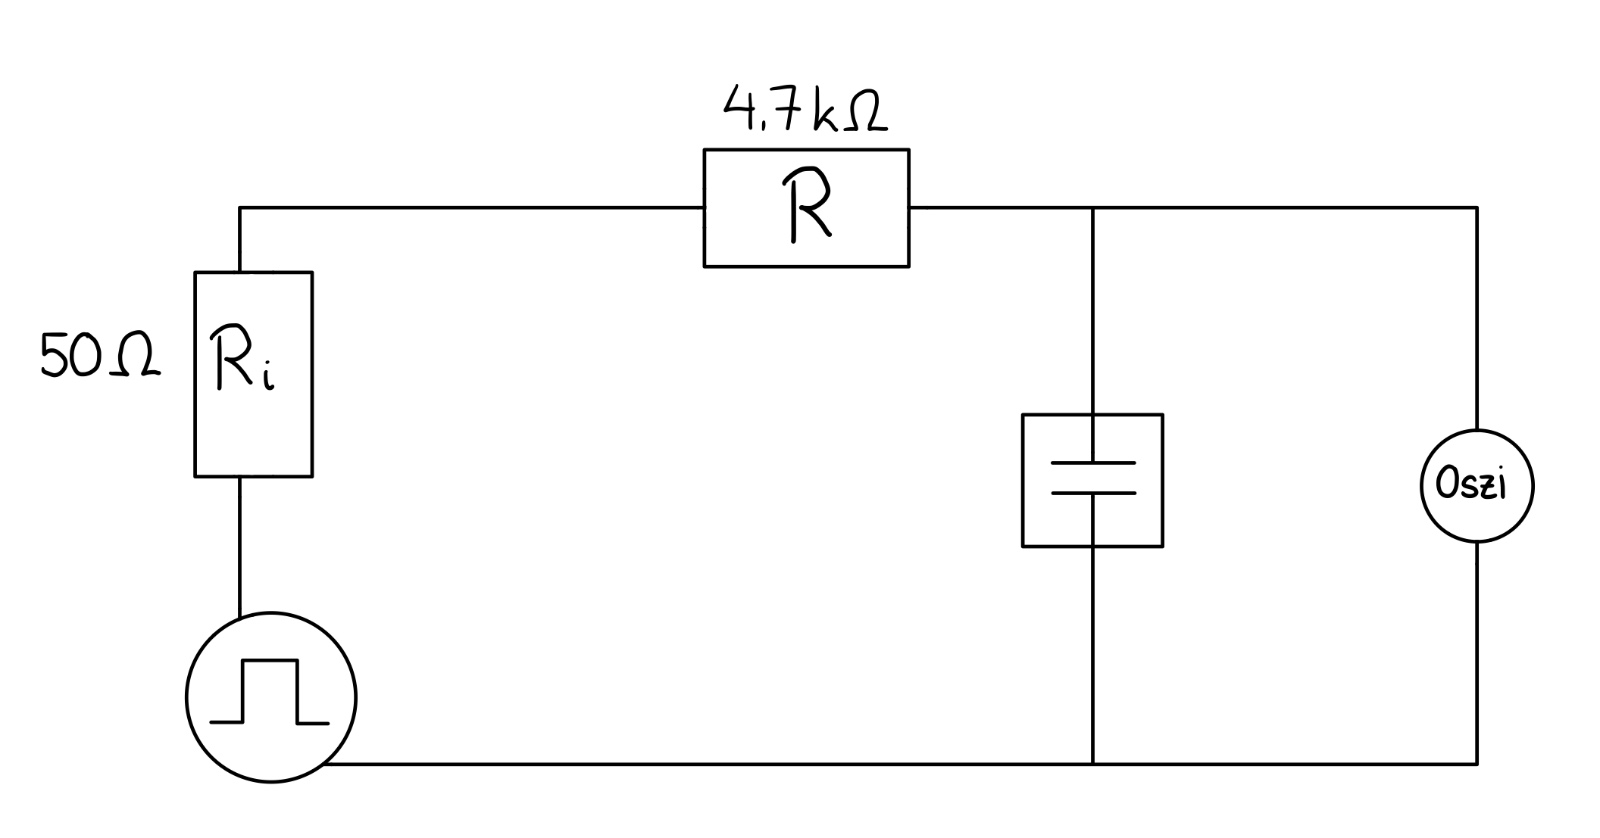
\includegraphics[width=0.6\textwidth]{../Quellen/Labor2/SchaltungsaufbauVersuch1.jpeg}
\caption{Schaltungsskizze}
\end{figure}

\noindent Für den Schatungsaufbau wurde zunächst der Funktionsgenerator mit einer BNC-Messleitung, mit Masse an die Black-Box Nr. 24 und mit der Versorgungsspannung an das Steckbrett angeschlossen. An den Anschluss, an dem die Versorgungsspannung anliegt, wurde ein Steckkabel angeschlossen, welches dann den 4.7~$\Omega$ in Reihe schält. Die Black-Box wurde nun ebenfalls mit dem Steckbrett, hinter den Widerstand, verschaltet. Das Oszilloskop wurde nun parallel zur Black-Box angeschlossen. Hierfür wurde ein Oszilloskop BNC Tastkopf mit Messklemme verwendet. Die Masseklemme wurde an die Black-Box-Masse verbunden. Die Messklemme wurde mit einem weiteren Steckkabel am Steckbrett eingehakt, welches parallel zum Kondensator verläuft. Der Schaltungsaufbau ist in Figure 3 dargestellt.

\begin{figure}[H]
    \centering
    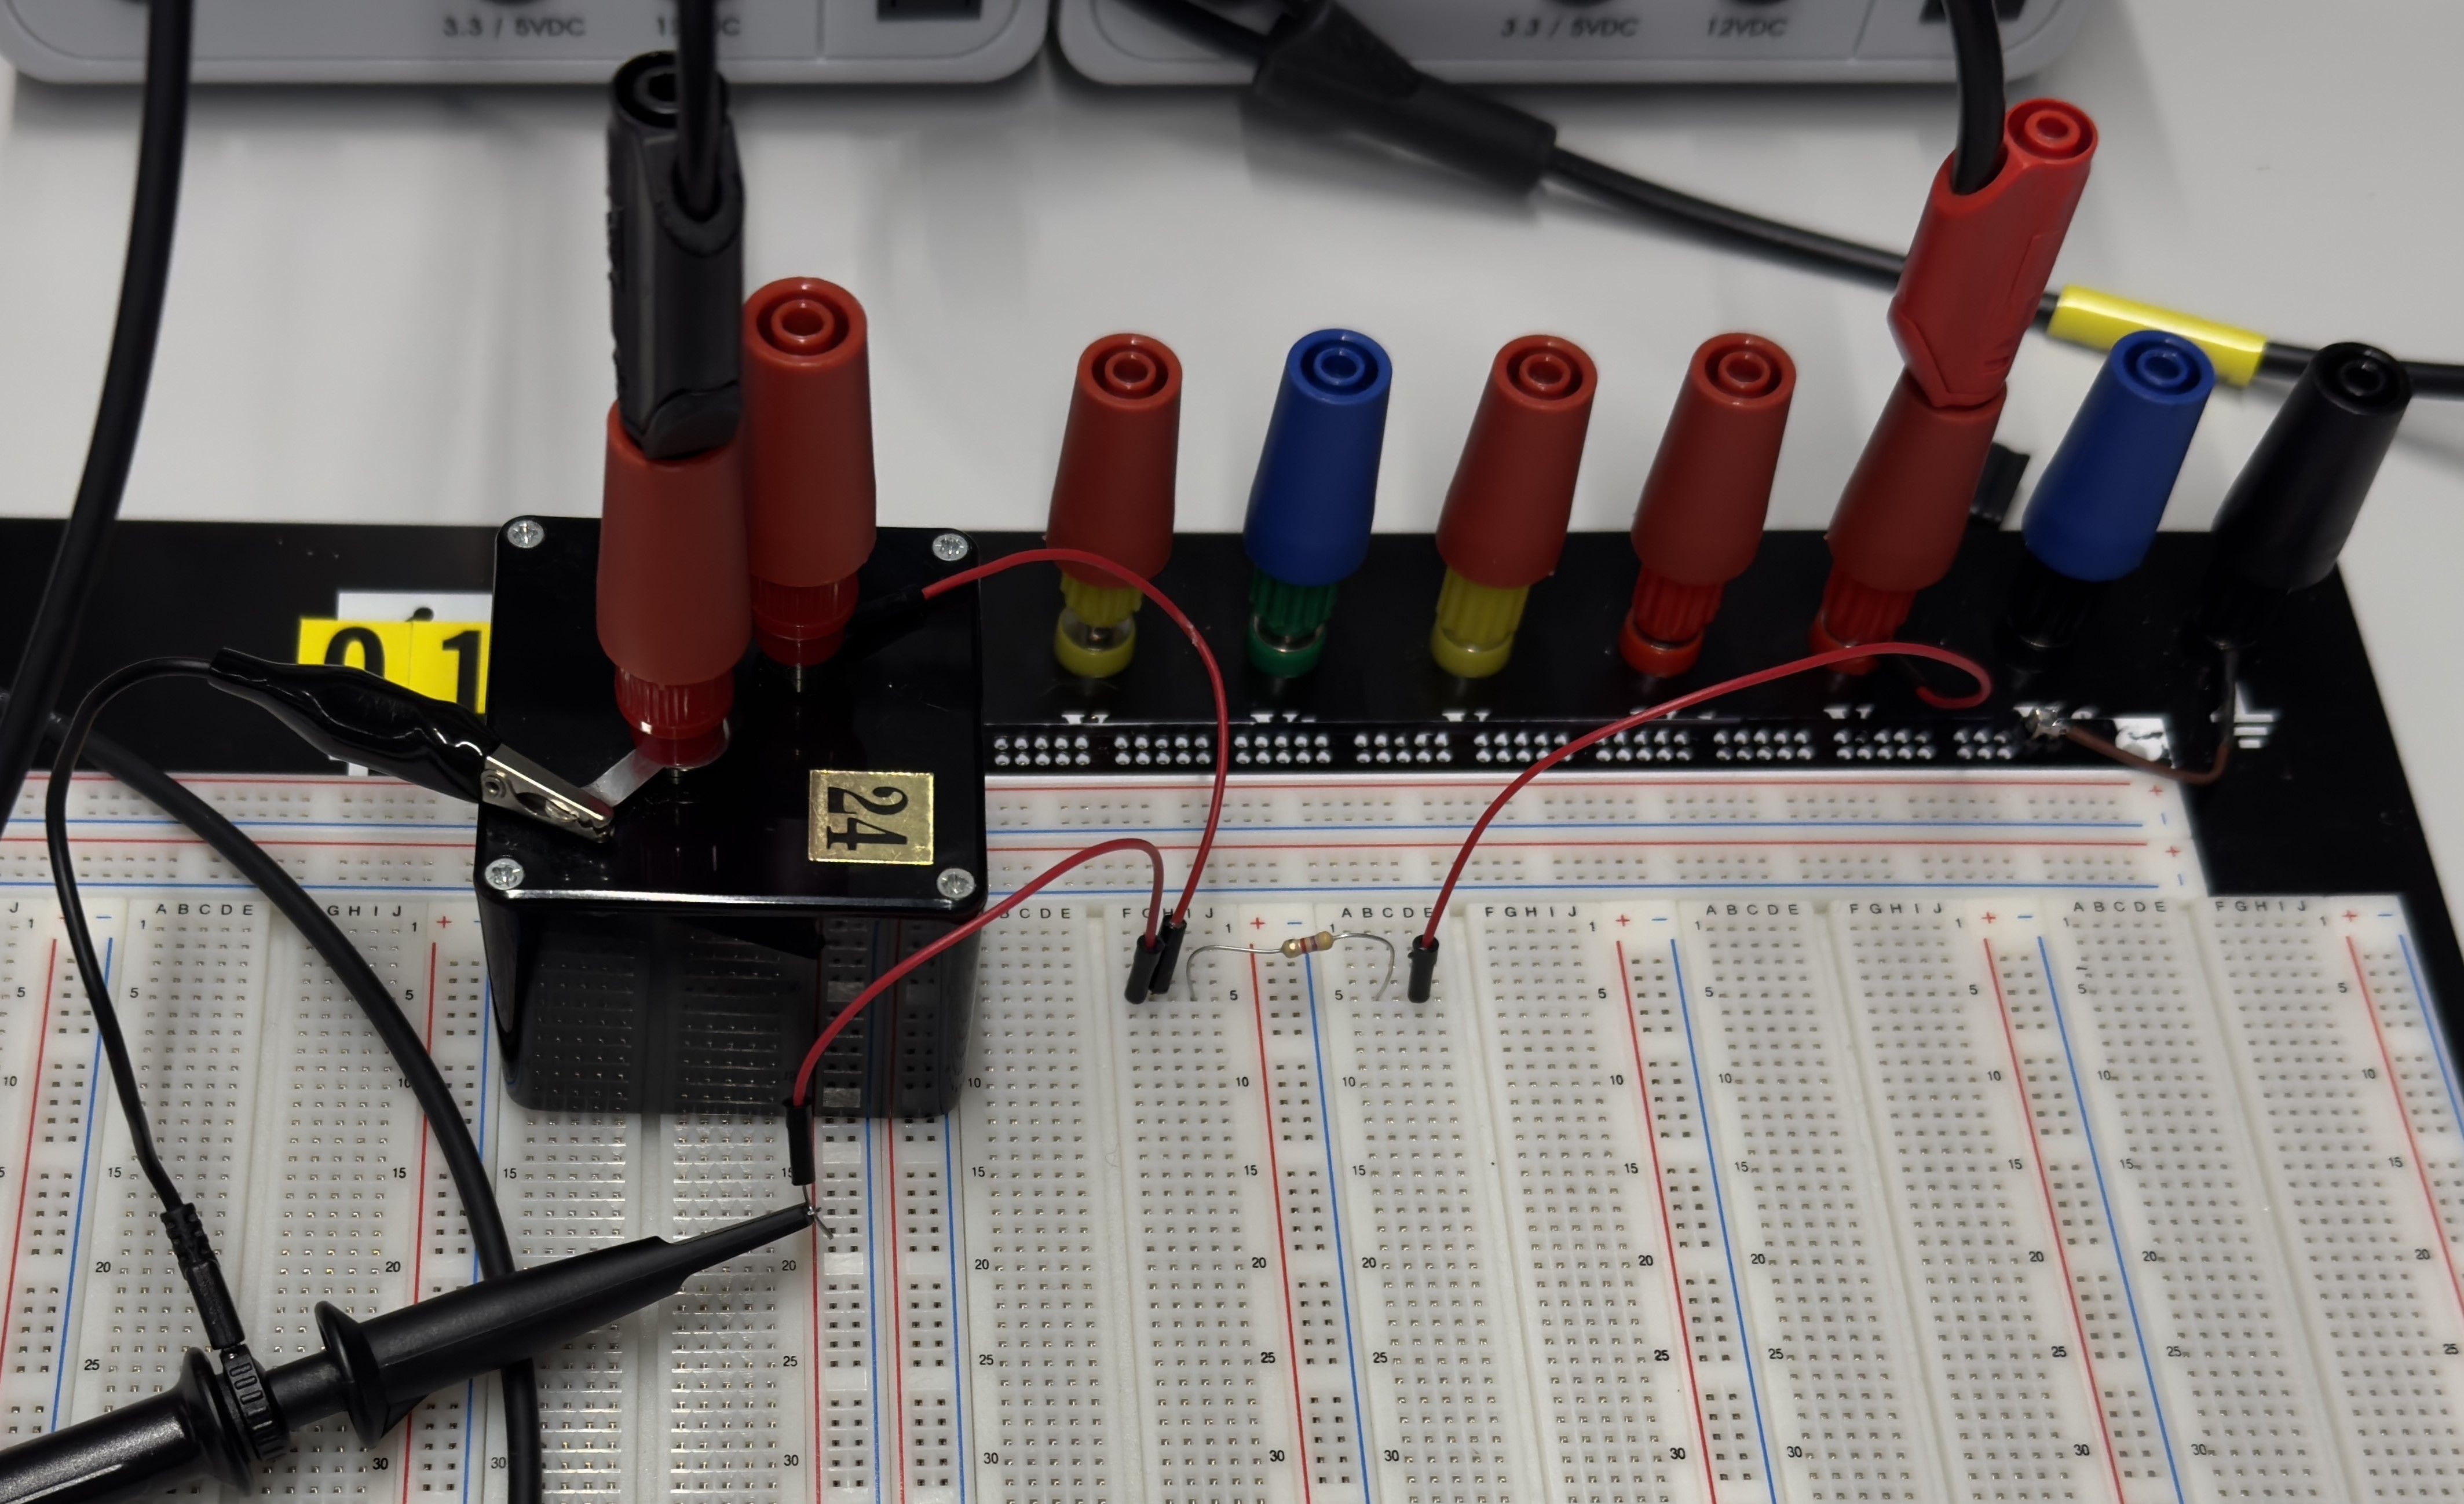
\includegraphics[width=0.7\textwidth]{../Quellen/Labor2/IMG_3965 - Kopie.jpeg}
\caption{Schaltungsaufbau}
\end{figure}

\noindent Der Verlauf der Lade- und der Entladekurve konnte nun am Oszilloskop abgelesen werden (siehe Figure 4). Nun sollte die Zeitkonstante Tau ($\tau$) ermittelt werden. Weil $\tau$ die Zeit angibt, die vergeht, bis ein Kondensator um 63~\% aufgeladen ist, wurde für die Ermittlung von $\tau$ die Eingangsspannung \(5~V \cdot 0.63~=~3.15~V\) gerechnet. Auf diesen Wert, wurden dann die Curser am Oszilloskop angepasst und das Bild geschickt vergrößert. Im sich ergebenden Bildabschnitt (siehe Figure 4), konnte nun die Zeit für $\tau$ abgelesen werden.\\\\
Anschließend an die Tau-Ermittlung sollte die Kapazität C\textsubscript{x} des Kondensators bestimmt werden. Hierzu wurde zuerst der ohm'sche Widerstand (4.7 k$\Omega$) mit dem Digital-Multimeter (DMM) nachgemessen. Der Widerstand wurde mit den Sicherheits-Klemmprüfspitzen, wie in Figure 5 gezeigt, gemessen. Mit diesem Widerstand, dem Innenwiderstand des Funktionsgenerators und der ermittelten Zeitkonstante konnte nun die Kapazität des Kondensators mit der Formel $\tau = R \cdot C$ ausgerechnet werden.\\
In Table 2 sind alle in der Schaltung und der Messanordnung vorkommenden absoluten bzw. relativen Einzelfehler aufgelistet.\\Einer der aufgelisteten Fehler, kommt durch das BNC-Kabel zustande. Dieses wirkt durch dessen Aufbau wie ein Kondensator. Die daraus resultierende, parasitäre Kapazität kann beispielsweise zu Signalverzerrungen führen. Um diesen Fehler zu vermeiden, beziehungsweise zu reduzieren, wurde ein Tastkopf verwendet. Tastköpfe sind für hochfrequente Signale und empfindliche Messungen besser geeignet und minimieren Verzerrungen und Signalverfälschungen.

\subsection{Messergebnisse}

\begin{figure}[H]
    \centering
    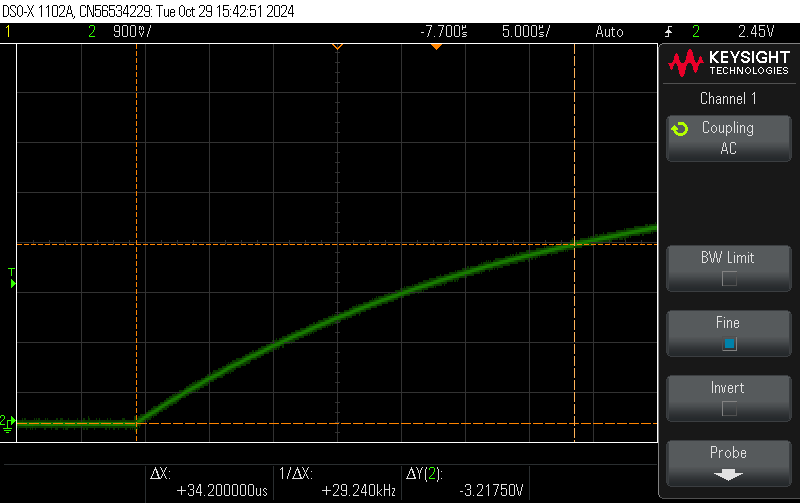
\includegraphics[width=0.8\textwidth]{../Quellen/Labor2/scope_1.png}
\caption{Ladekurve des Kondensators}
\end{figure}
Aus der Ladekurve in Figure 4 konnte für Tau, unter $\Delta X$, der Wert \(\tau~=~34.2~\cdot~10^{-6}~s\) abgelesen werden.\\

\begin{figure}[H]
    \centering
    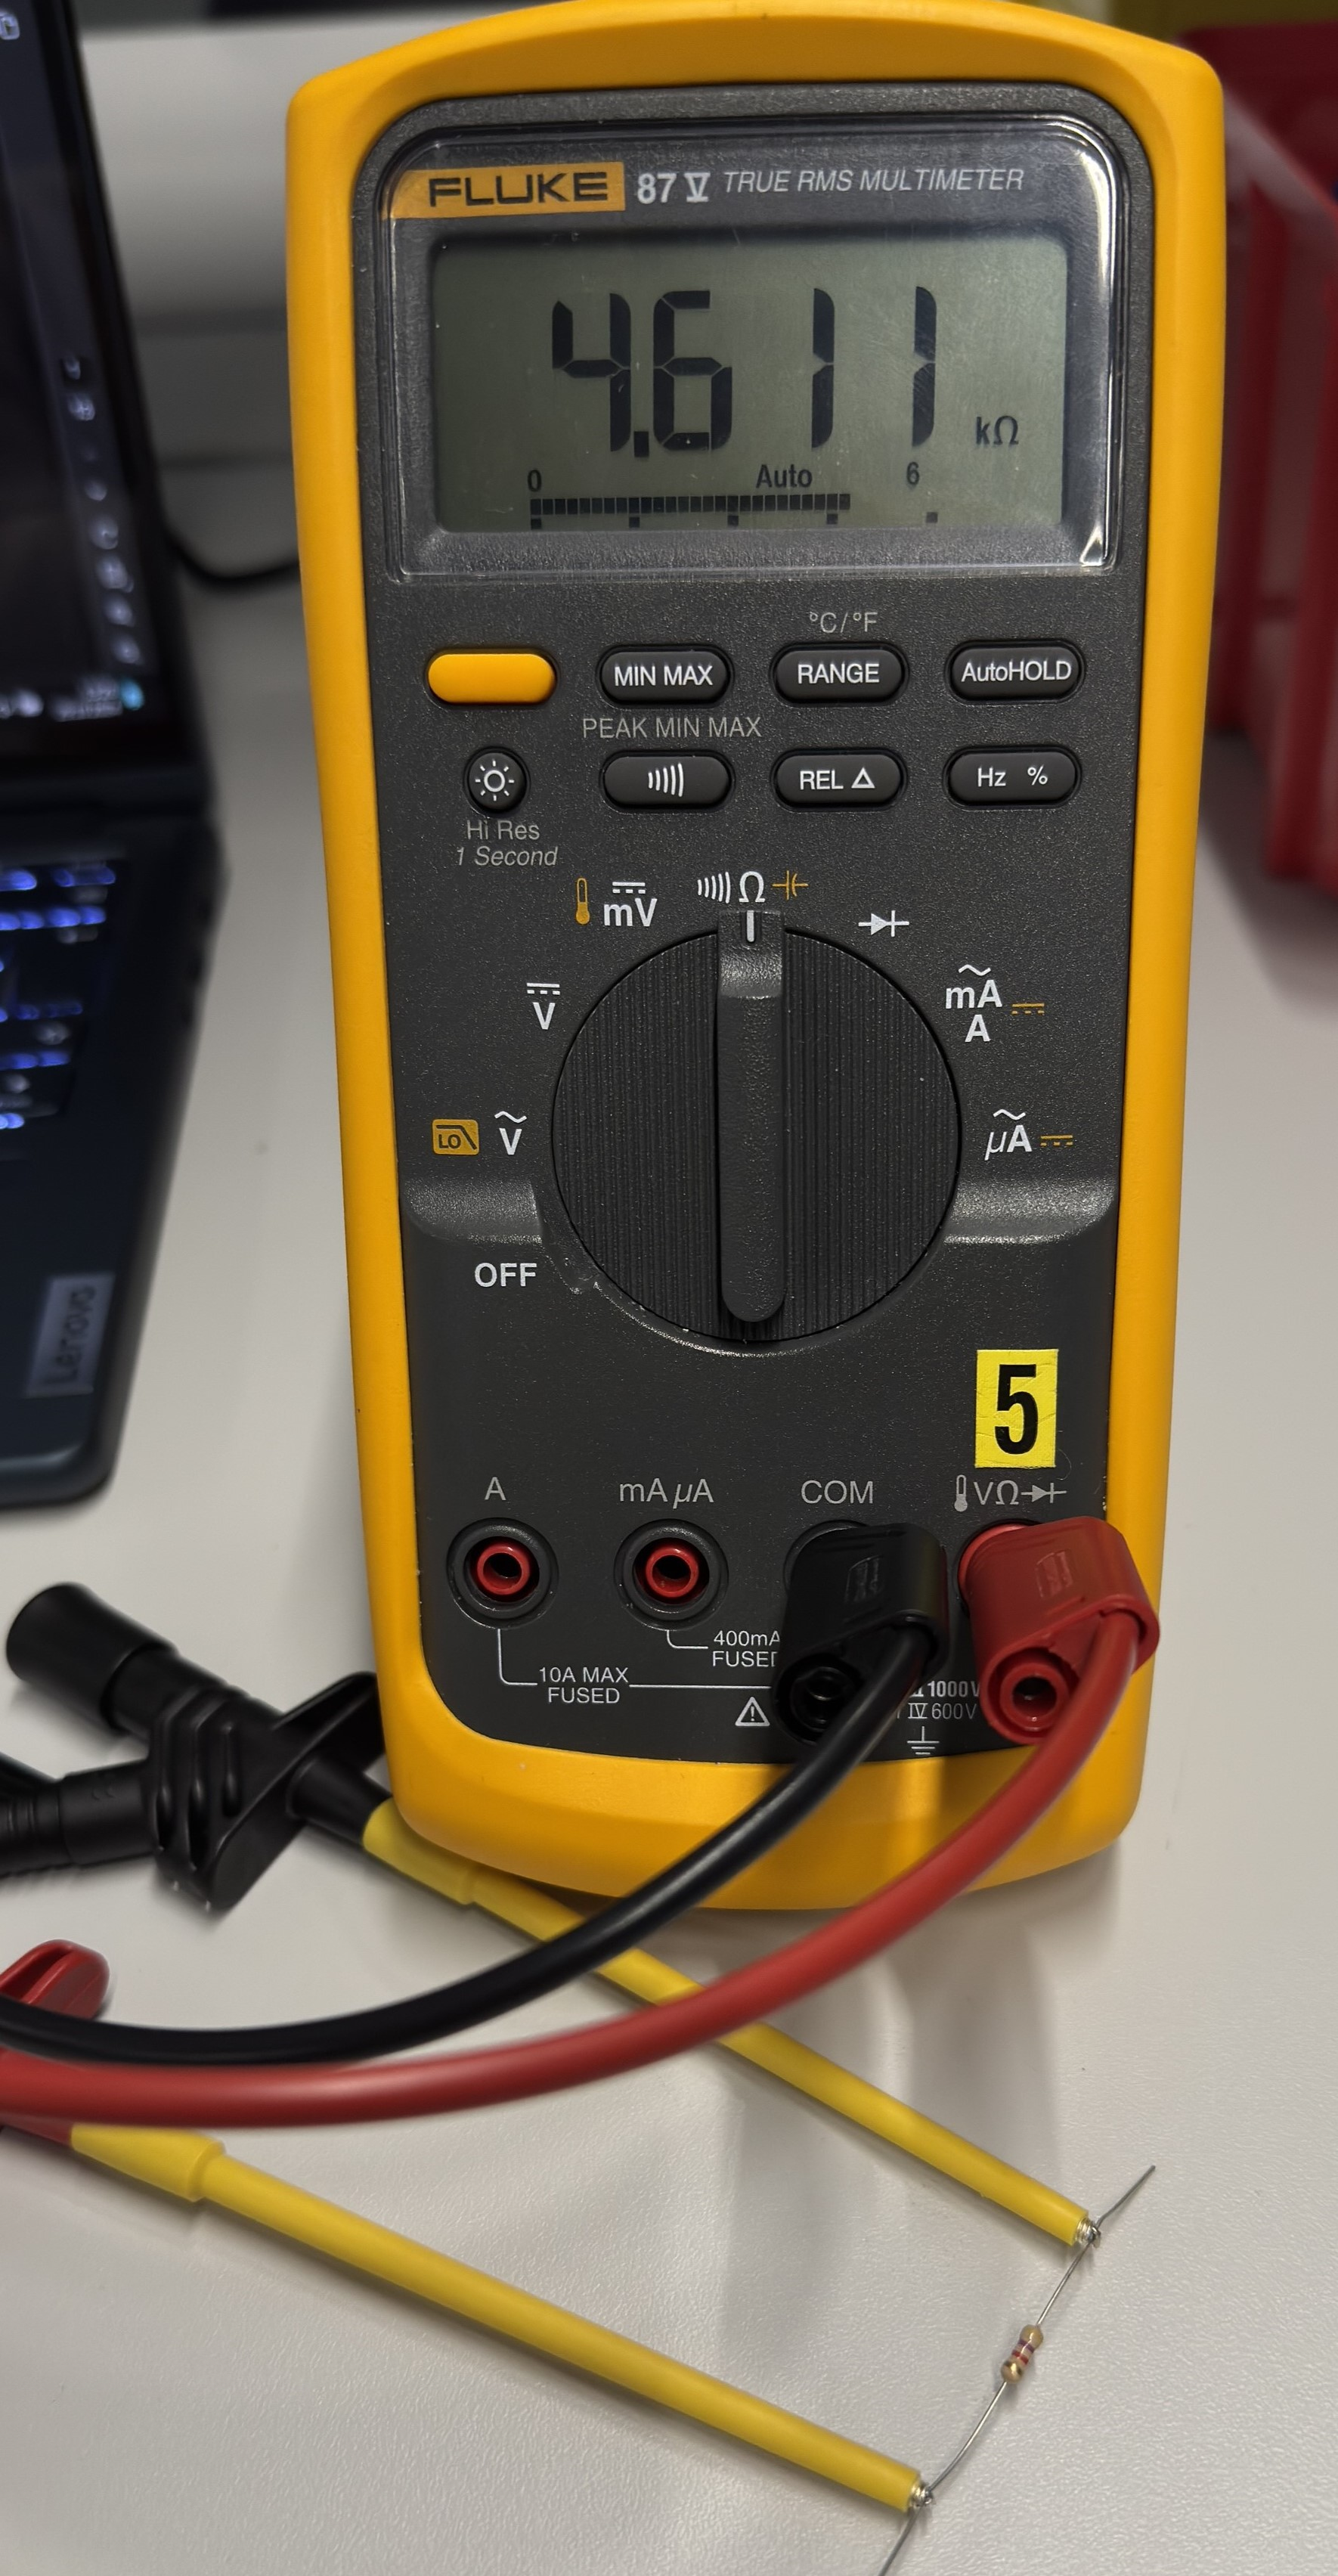
\includegraphics[width=0.3\textwidth]{../Quellen/Labor2/Fotos/IMG_3963gezoomt.jpeg}
\caption{Messung ohm'scher Widerstand mit dem DMM}
\end{figure}

\noindent In die genannte Formel, wurde für R der gemessene Widerstand mit 4611~$\Omega$, mit dem 50~$\Omega$ Innenwiderstand addiert. Das, aus Figure 4, abgelesene $\tau$ wurde eingesetzt und die Formel ausgerechnet.
\[
C\textsubscript{x} ~=~ \frac{\tau}{R} ~=~ \frac{34.2 \cdot 10^{-6}s}{4611~\Omega + 50~\Omega} ~\approx~ 7.337~nF
\]
\noindent Als Kapazität für den Kondensator ergab sich dadurch ein Wert von 7.337~$nF$.\\
Wird mit dem Nominalwert und der Toleranz, anstelle dem gemessenen Widerstands-Wert gerechnet, ergibt sich Folgendes:
\[
C\textsubscript{x} ~=~ \frac{\tau}{R} ~=~ \frac{34.2 \cdot 10^{-6}s}{4700~\Omega~\pm(4700~\Omega~\cdot~0.05) + 50~\Omega}
\]

\[
C\textsubscript{x1}~\approx~ 6.861~nF~~~~~~~~~~~~~
C\textsubscript{x2}~\approx~ 7.575~nF
\]

\noindent Bei Addition der Toleranz, ergibt die Rechnung nur knappe 94~\% der, mit dem gemessenen Widerstand errechneten, Kapazität, also 6~\% und 476~$\mu F$ weniger. Wird die Toleranz subtrahiert, ergeben sich 103~\% der Kapazität und damit 3~\% und 238~$\mu F$ mehr.
\textcolor{red}{Hat dies einen Einfluss auf die Genauigkeit des Ergebnisses von Cx und auf seinen Gesamtfehler, und wenn ja, welchen?}

\begin{table}[H]
	\centering
	\scalebox{0.8}{	
\begin{tabular}{|c|c|c|c|c|c|}
		\hline
		\textbf{Fehlerquelle} & \textbf{Einfluss} & \textbf{typische Größe} & \textbf{stat. oder sys.} & \textbf{Berücksichtigung?} & \textbf{relevant?}\\
		\hline
		R = 4.7 k$\Omega$ & DMM-Messung & \textperthousand ~siehe Datenblatt & statistisch & Fehlerrechnung & Ja\\
		\hline
		Oszilloskop & R\textsubscript{i},C\textsubscript{i} Tastkopf (10x) & 10 µ$\Omega$, $\sim$pF & systematisch & Nein \( < 0.5 \)\textperthousand & Nein\\
		  & x, y - Messung & \(\approx 3\) \% Datenblatt! & statistisch & Fehlerrechnung & Ja\\
		  & Curser & Steigung beachten & statistisch & Fehlerrechnung & Ja\\
		\hline
		Funktionsgenerator & Anstiegszeit & einige ns & systematisch & \( \approx 1 \) \textperthousand & Nein\\
		  & R\textsubscript{i} & 50 $\Omega$ & systematisch & Korrektur & Ja\\
		  &   & $\Delta R$\textsubscript{i} (\(\approx 1\)\%) & statistisch & 1$\%$ \( \Rightarrow\) $\pm ~0.5~\Omega$ & Nein\\
		  & Amplitude, Offset & - & systematisch & relativ & Nein\\
		\hline
		Kabel +5 V & Widerstand & \(\approx 20\)m$\Omega$ & systematisch & zu klein & Nein\\
		\hline
	\end{tabular}
	}
	\caption{Vorkommende Einzelfehler}
\end{table}

\subsubsection* {Fehler DMM - Messung}
\[
\Delta R~=~\pm(4.611~k\Omega~\cdot~0.02~\%~+~0.001~k\Omega)~=~\pm~1.94~\Omega
\]
\[
R\textsubscript{-}~=~4609.06~\Omega~~~~~~~~~~R\textsubscript{+}~=~4612.94~\Omega
\]

\subsubsection* {Fehler x, y - Messung}
\underline{Vertikale Messungenauigkeit:}\\\\
Vertical gain accuracy: 
\[
+(3~\% \cdot 8 \cdot 900~mV)~=~+( 0.03 \cdot 7200~mV)~=~+~216~mV
\]
Dual cursor accuracy: 
\[
\Delta U~=~\pm[DC~vertical~gain~accuracy + 0.5~\%~full~scale]
\]
\[
\Delta U~=~\pm~216~mV~+~0.5~\%~\cdot~7200~mV~=~\pm~252~mV
\]
\noindent \underline{Horizontale Messungenauigkeit:}\\\\
$\Delta$ Time accuracy:
\[
\Delta t~=~\pm(100~ppm~\cdot~34.2~\mu s~+~0.0016~\cdot~5~\mu s~+~0.2~\mu s)~=~\pm(3.42~ns~+~8~ns+0.2~ns)~=~\pm~11.62~ns
\]


\subsubsection* {Fehler Curser}
\underline{Einstellungenauigkeit der Curser:}\\\\
-horizontal: \(\frac{5~\mu s}{div}\)~=~\(\frac{5~\mu s}{50}\)~=~100 ns~~~~~~~~~~~~~~
+vertikal: \(\frac{0.9~V}{div}\)~=~\(\frac{0.9~V}{7.2}\)~=~12.5~mV\\\\
\underline{Einfluss der vertikalen Messungenauigkeit auf die Messung der Zeitkonstante:}\\
\[
m\textsubscript{$\tau$}~=~\frac{dU\textsubscript{C}}{dt}~=~\frac{U\textsubscript{0}}{e~\cdot~\tau}~=~\frac{5~V}{e~\cdot~34.2~\mu s}~\approx~53.78~\frac{V}{ms}
\]
\[
\Delta t\textsubscript{v}~=~\frac{252~mV}{53.78~\frac{V}{ms}}~\approx~4.69~\mu s
\]
\[
\Delta t~=~\pm(4.69~+~ 0.01162)~\mu s~\approx~\pm~4.70162~\mu s
\]
\underline{Messergebnis:}
\[
\tau~=~(34.2~\pm~4.70162)~\mu s~~~~~bzw.~~~~~\tau~=~(34.2~\mu s~\pm~13.75\%)
\]
\subsubsection* {Wahrscheinlicher Fehler}
\[
\Delta C\textsubscript{wahrsch.}=\sqrt{\left(\frac{\Delta \tau}{R}\right)^2+\left(\frac{\tau\cdot\Delta R}{R^2}\right)^2}=\sqrt{\left(\frac{4.70162~\mu s}{4611~\Omega}\right)^2+\left(\frac{34.2~\mu s\cdot1.94~\Omega}{(4611~\Omega)^2}\right)^2}=\pm~1019.658~ pF
\]

\[
\Delta C\textsubscript{wahrsch.-relativ}~=~\frac{\Delta C\textsubscript{wahrsch.}}{C\textsubscript{x}}~=~\frac{1019.658~pF}{7.337~nF}~=~13.9~\%
\]


\subsubsection* {Größtfehler}
\[
\Delta C\textsubscript{max.}~=~\left\lvert \frac{\Delta \tau}{R}\right\rvert+\left\lvert \frac{\tau~\cdot~\Delta R}{R^2}\right\rvert~=~\left\lvert \frac{4.70162~\mu s}{4611~\Omega}\right\rvert+\left\lvert \frac{34.2~\mu s~\cdot~1.94~\Omega}{(4611~\Omega)^2}\right\rvert~=~1022.774~pF
\]

\[
\Delta C\textsubscript{max.-relativ}~=~\frac{\Delta C\textsubscript{max.}}{C\textsubscript{x}}~=~\frac{1022.774~pF}{7.337~nF}~=~13.94~\%
\]



\newpage
\section{Versuch 2: Passiver Zweipol (Black Box)}
\subsection{Zielsetzung}
Das Ziel des zweiten Versuchs, ist die Bestimmung der Bauteil-Typen (Möglichkeiten: R, L oder C) und deren Anordnung innerhalb einer
Black Box.

\subsection{Bauteile und Messgeräte}
\subsubsection*{Messgeräte}
\begin{itemize}
\item Teledyne Technologies Funktionsgenerator T3AFG80 80 MHz
\item Keysight Oszilloskop (DSOX1102A)
\item Netzgerät (NEP-8323)
\item Fluke 87 V True RMS Multimeter
\item Oszilloskop BNC Tastkopf mit Messklemme
\item Steckkabel (mehrere)
\item Tru Components Steckbrett
\item Bananenkabel (schwarz und rot)
\item Sicherheits-Klemmprüfspitze (2 Stück)
\end{itemize}

\subsubsection*{Bauteile}
\begin{itemize}
\item Black-Box (Nr. 1-17)
\item Widerstand Nominalwert 4,7 k$\Omega$
\end{itemize}




\subsection{Messkonzept}
Der Schaltungsaufbau des ersten Versuchs konnte so beibehalten werden. Es musste lediglich die Black-Box des ersten Versuchs durch eine Black-Box mit einer Nummer zwischen 1 und 17 ersetzt werden. In diesem Versuchsbericht wurde Nummer 6 verwendet. Diese Black-Box konnte identisch zur Vorherigen angeschlossen werden. Um herauszufinden, welche Bauteile sich in der Black-Box befinden und wie diese miteinander verschaltet sind, sollten die Frequenzen des Rechtecksignals verändert werden und dabei der Verlauf der Funktion auf dem Oszilloskop beobachtet werden.\\
An dem Verlauf, welcher in Figure 7 zu sehen ist, konnte mithilfe der Curser abgelsen werden, dass die Eingangsamplitude 5 V und die Ausgangsamplitude 2,96 V entspricht. Dazu kommt, dass es sich um ein periodisches Verhalten handelt und ein Lade- und ein Entladevorgang erkennbar sind. Daraus lässt sich schließen, dass es sich in jedem Fall um einen Kondensator handeln muss. Durch die Widerstands-Messung der Black-Box durch ein DMM, wurde ein Widerstand von \(6.74~k\Omega\) festgestellt. Daraus ließ sich schließen, dass sich in der Black-Box, neben dem Kondensator, auch ein Widerstand befinden muss. Es konnte am Oszilloskop beobachtet werden, dass auch bei 0~Hz noch eine Spannung an der Black-Box anliegt. Wäre der Widerstand in Reihe zum Kondensator geschalten, würde der Kondensator bei 0~Hz keine Spannung durchlassen. Daraus lässt sich schließen, dass es sich um eine Parallelschaltung handeln muss.
\\Nun sollte die Größe der Bauelemente bestimmt werden. Hierfür wurde der Widerstand der Black-Box mit dem DMM gemessen (siehe Figure 8). Die Größe des Kondensators konnte anschließend mithilfe des Gesamtwiderstands, ermittelt aus Innenwiderstand des Funktionsgenerators, Vorwiderstand und Black-Box-Widerstand, sowie der Zeitkonstante~$\tau$ berechnet werden.\\
\noindent Das Rechteck-Eingangssignal am Ausgang des Zweipols vezerrt. Um mit dem Oszilloskop einen, zur Eingangsspannung proportionalen, Signalverlauf darzustellen, musste ein Kondensator parallel zum Vorwiderstand R\textsubscript{V} geschalten werden (siehe Figure 6).

\begin{figure}[H]
    \centering
    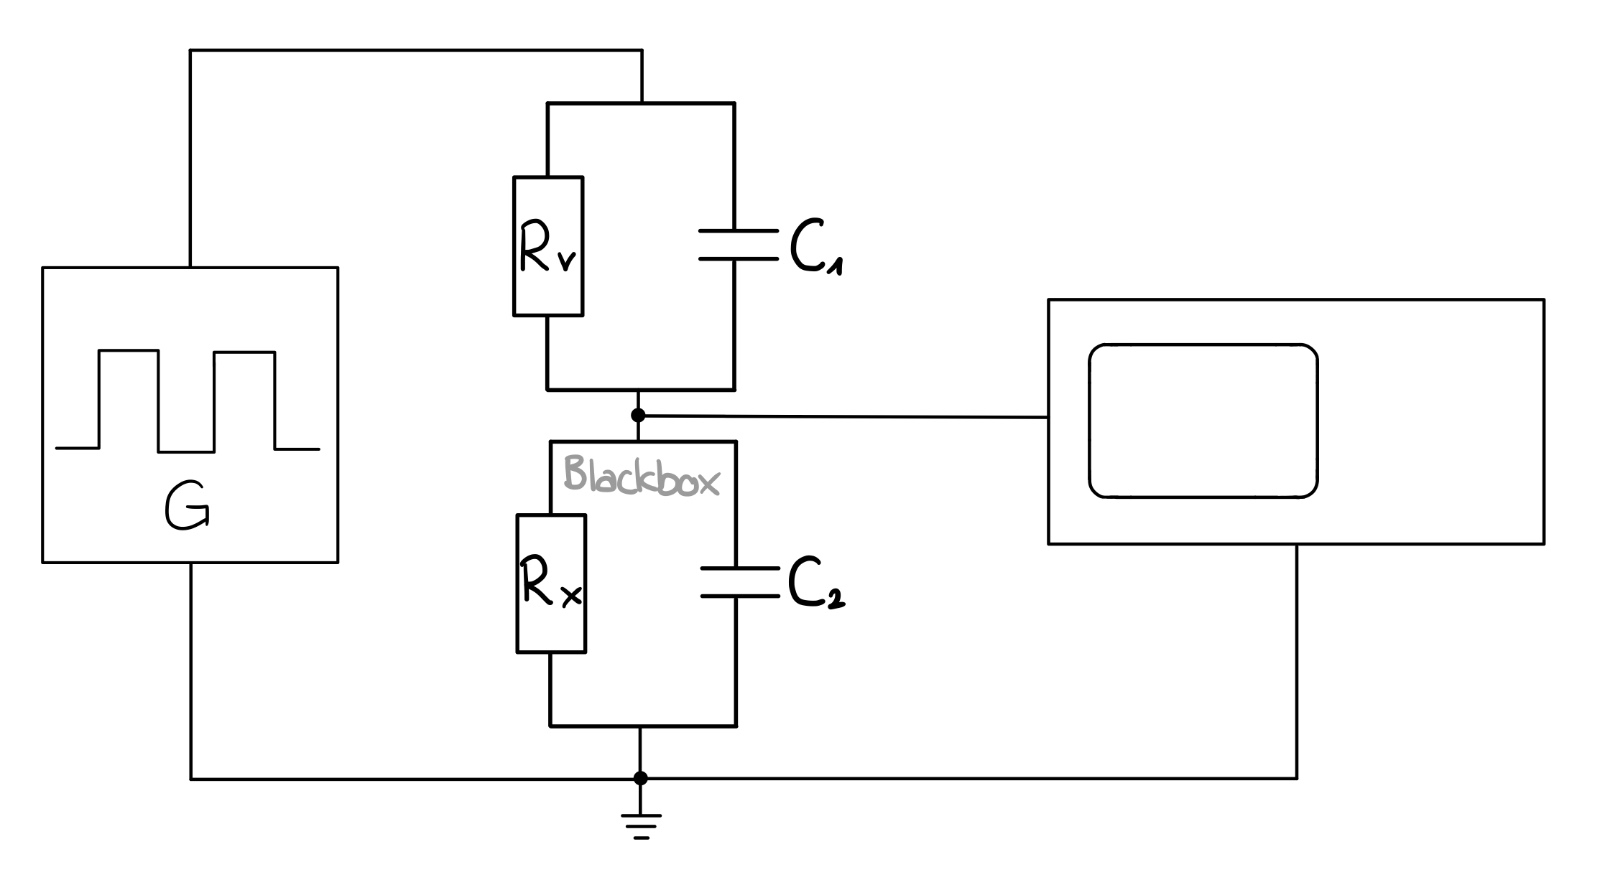
\includegraphics[width=0.7\textwidth]{../Quellen/Labor2/SkizzeVerschaltungWiderstandKondensatorVersuch2.jpeg}
\caption{Schaltskizze}
\end{figure}

\noindent Dieses Verfahren wird Kompensation genannt. Es wird allgemein verwendet, um Messfehler und Ungenauigkeiten zu eliminieren. Besonders bei elektrischen und mechanischen Messgeräten, sowie auch bei thermischen Messungen kommt die Kompensation häuig zum Einsatz.\\


\noindent Das Verhältnis der Widerstände muss gleich dem Verhältnis der Impedanzen der Kondensatoren sein. Mit diesem Wissen konnte die Größe dieses Kondensators wie folgt berechnet werden:
\[
\frac{C\textsubscript{2}}{C\textsubscript{1}}~=~\frac{R\textsubscript{v}}{R\textsubscript{x}}~=~\frac{4.7~k\Omega}{6.74~k\Omega}~\approx~0.673\]

\[
C\textsubscript{1}~=~\frac{C\textsubscript{2}}{0.673}~=~\frac{5088.93~pF}{0.673}~\approx~7297.742~pF
\]



\noindent Wie bereits bei Versuch 1 beschrieben wurde, kann die Verwendung eines BNC-Kabels, durch dessen Aufbau, zu Signalverfälschungen führen. Daher wurde auch mit mit einem Tastkopf gemessen, um diese zu verringern.


\subsection{Messergebnisse}
\begin{figure}[H]
    \centering
    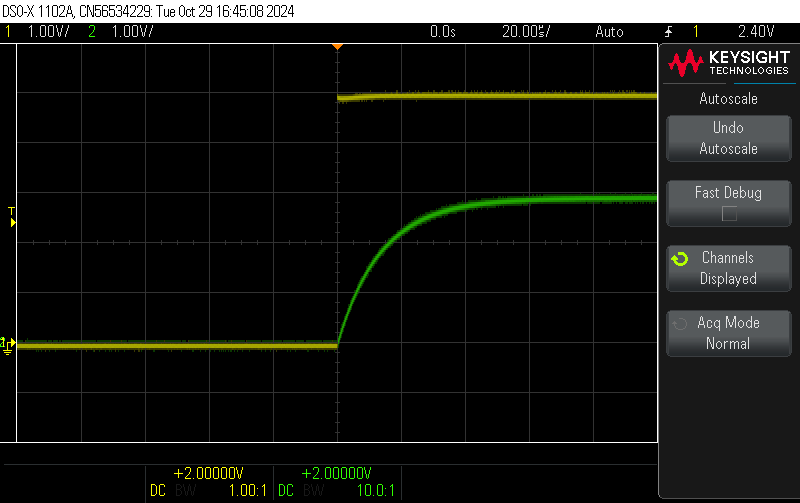
\includegraphics[width=0.7\textwidth]{../Quellen/Labor2/scope_3.png}
\caption{Verlauf Funktion der Black-Box}
\end{figure}



\begin{figure}[H]
    \centering
    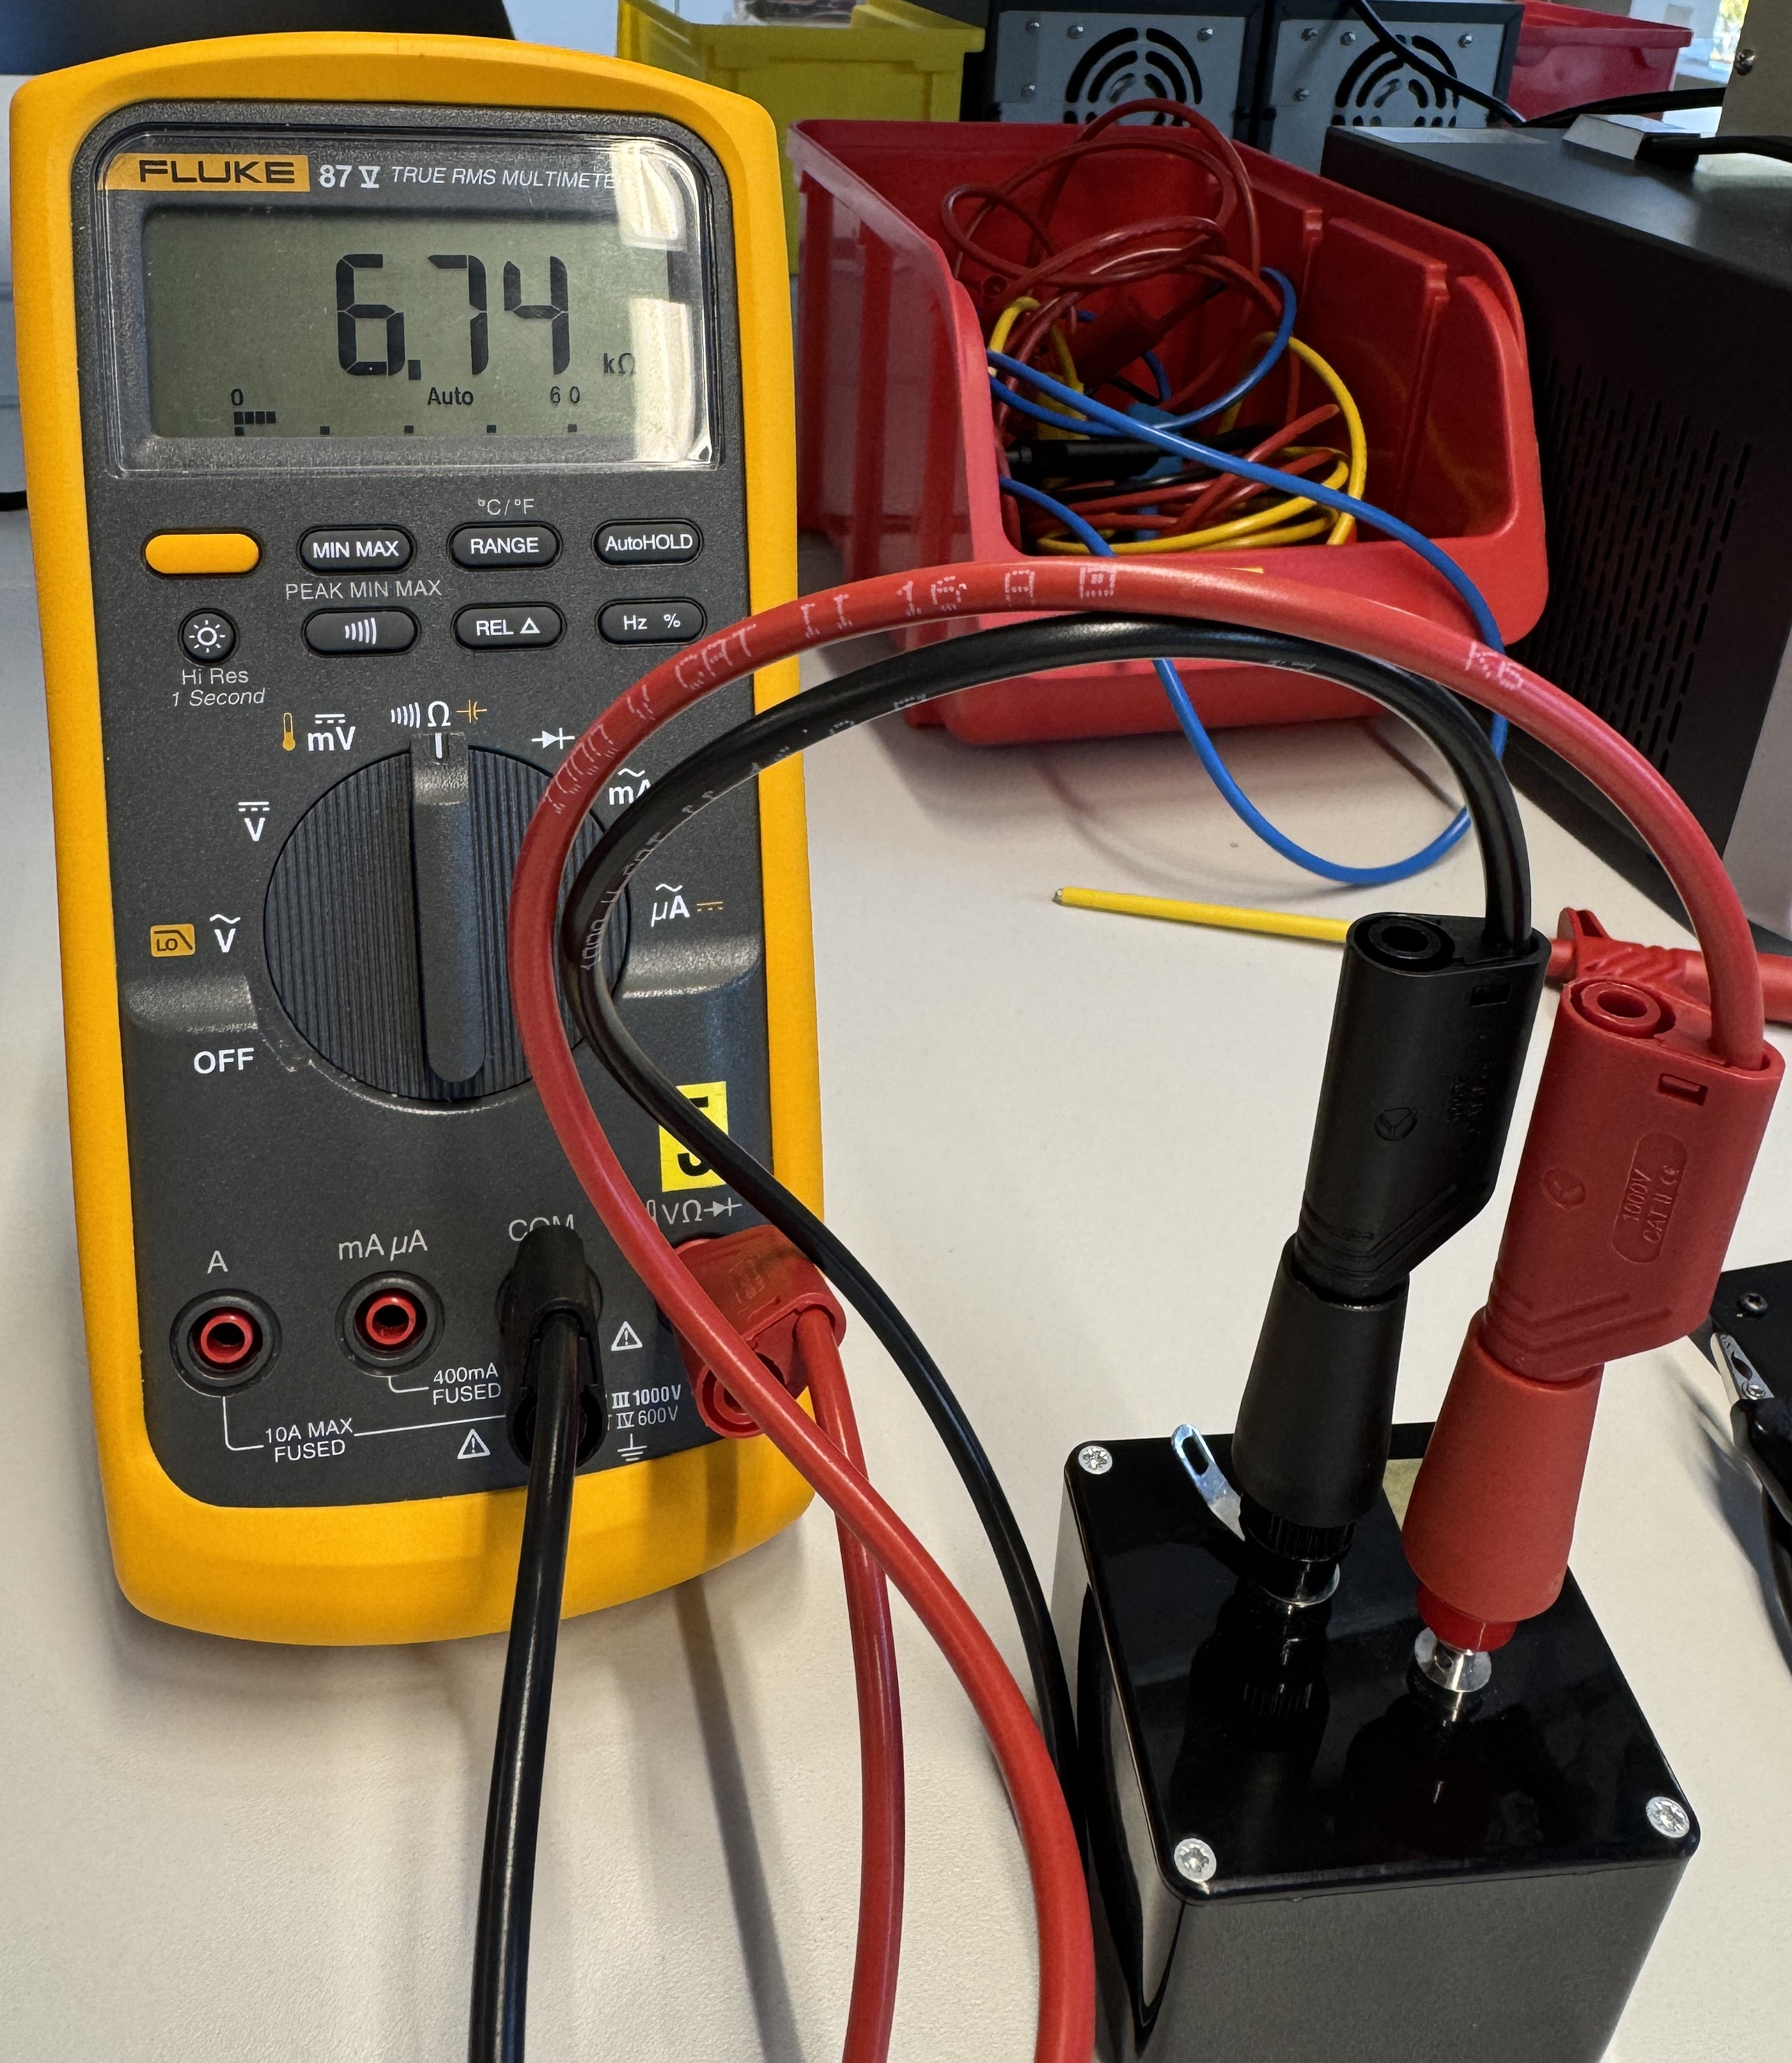
\includegraphics[width=0.4\textwidth]{../Quellen/Labor2/Fotos/IMG_3973gezoomt.jpeg}
\caption{Widerstandmessung der Black-Box~~~R~=~6.74~k$\Omega$}
\end{figure}


\noindent Wie im Messkonzept bereits beschrieben, wurde für die Kapazitäts-Bestimmung des Kondensators zunächst der Gesamtwiderstand ausgerechnet.
\[
R\textsubscript{ges}~=~\frac{R\textsubscript{1} \cdot R\textsubscript{2}}{R\textsubscript{1}~+~R\textsubscript{2}}~=~\frac{(50~\Omega~+~4611~\Omega) \cdot 6740~\Omega}{(50~\Omega~+~4611~\Omega)~+~6740~\Omega}~=~2.755~k\Omega
\]
Um die Kapazität nun mit der Formel \(C=\frac{\tau}{R}\) auszurechnen, wurde noch der Wert für Tau benötigt. Dieser konnte wie bei Versuch 1 am Oszilloskop abgelesen werden: $\tau~=~14.02~\mu s$. Daraus ergibt sich folgende Rechnung:
\[
C~=~\frac{\tau}{R}~=~\frac{14.02~\mu s}{2.755~k\Omega}~=~5088.93~pF
\]





\newpage
\section{Versuch 3: Leistungsaufnahme eines elektrischen Widerstands}
\subsection{Zielsetzung}
In diesem Versuch soll die elektrische Leistung bestimmt werden, die bei Stromdurchfluss in
einem Widerstand R anfällt. Es werden zwei Verfahren verglichen, mit dem Ziel das Verfahren zu ermitteln, mit dem eine genauere Bestimmung möglich ist.

\subsection{Bauteile und Messgeräte}
\subsubsection*{Messgeräte}
\begin{itemize}
\item Netzgerät (NEP-8323)
\item Fluke 87 V True RMS Multimeter
\item Steckkabel (mehrere)
\item Tru Components Steckbrett
\item Bananenkabel (schwarz und rot)
\item Sicherheits-Klemmprüfspitze (2 Stück)
\end{itemize}

\subsubsection*{Bauteile}
\begin{itemize}
\item Widerstand Nominalwert 1 k$\Omega$ (2 Stück)
\end{itemize}





\subsection{Messkonzept}
Zu Beginn dieses Versuchs, wurden die beiden Widerstände mit dem DMM nachgemessen (siehe Table 3), um die Genauigkeit der darauf folgenden Messungen zu steigern. Anschließend wurde das Netzgerät auf 5~V Spannung eingestellt und der Strom auf 200~mA begrenzt. Gemäß der Schaltskizze~1 (siehe Figure 9) wurde nun eine Schaltung aufgebaut (siehe Figure 10). Das Netzgerät versorgt das Steckbrett mit der voreingestellten Spannung. Der Strom wurde nun mit den Sicherheits-Klemmprüfspitzen mittels direkter Strommessung auf 5.06~mA bestimmt (siehe Figure 10). Über die Formel \(P = I^2 \cdot R \) konnte nun die Leistung bestimmt werden.

\[
P ~=~ I^2 \cdot R ~=~ (5.06~mA)^2 \cdot 988~\Omega ~=~ 25.3~mW
\]\\
Einzelne Fehlerbeiträge:
\[
\Delta I~=~\pm(0.2~\%~\cdot~5.06~mA~+~0.04~mA)~=~\pm~50.12~\mu A
\]
\[
\Delta R~=~\pm(988~\Omega~\cdot~0.02~\%~+~1\Omega)~=~\pm~1.198~\Omega
\]
Wahrscheinlicher Messfehler:\\
\[
\Delta P\textsubscript{wahrsch.}~=~\sqrt{\left(2~I~\cdot~R~\cdot~\Delta I\right)^2~+~\left(I^2~\cdot~\Delta R\right)^2}
\]
\[
=~\sqrt{\left(2~\cdot~5.06~mA~\cdot~988~\Omega~\cdot~50.12~\mu A\right)^2~+~\left((5.06~mA)^2~\cdot~1.198~\Omega\right)^2}~=~\pm~502.066~\mu W
\]\\
\[
\Delta P\textsubscript{wahrsch.-relativ}~=~\frac{\Delta P\textsubscript{wahrsch.}}{P}~=~\frac{502.066~\mu W}{25.3~mW}~\approx~1.98~\%
\]
Größtfehler:\\
\[
\Delta P\textsubscript{max.}~=~\left\lvert 2~I~\cdot~R~\cdot~\Delta I\right\rvert~+~\left\lvert I^2~\cdot~\Delta R\right\rvert
\]
\[
=~\left\lvert 2~\cdot~5.06~mA~\cdot~988~\Omega~\cdot~50.12~\mu A\right\rvert~+~\left\lvert (5.06~mA)^2~\cdot~1.198~\Omega\right\rvert~=~\pm~531.801~\mu W
\]\\
\[
\Delta P\textsubscript{max.-relativ}~=~\frac{\Delta P\textsubscript{max.}}{P}~=~\frac{531.801~\mu W}{25.3~mW}~\approx~2.1~\%
\]\\


\noindent Nun wurde die Versorgungsspannung auf 10~V erhöht. Die Schaltung wurde gemäß der Schaltskizze~2 (siehe Figure 9) umgebaut (siehe Figure 11). Nun sollte mit indirekter Strommessung gemäß der Formel \(P ~=~  (\frac{U}{R\textsubscript{V}})^2 \cdot R\) die Leistung bestimmt werden. Dabei soll r\textsubscript{v} als zweiter Widerstand dienen.

\[
P ~=~  \left(\frac{U}{R\textsubscript{V}}\right)^2 \cdot R ~=~ \left(\frac{10~V}{996~\Omega}\right)^2 \cdot 988~\Omega ~\approx~ 99.6~mW
\]\\

\noindent Einzelne Fehlerbeiträge:
\[
\Delta U~=~\pm(0.05~\%~\cdot~10~V~+~0.01~V)~=~\pm~15~mV
\]
\[
\Delta R\textsubscript{V}~=~\pm(996~\Omega~\cdot~0.02~\%~+~1\Omega)~=~\pm~1.1992~\Omega
\]
Wahrscheinlicher Messfehler:\\
\[
\Delta P\textsubscript{wahrsch.}~=~\sqrt{\left(\left(\frac{U}{R\textsubscript{V}}\right)^2~\cdot~\Delta R\right)^2~+~\left(-\frac{2~U^2}{R\textsubscript{V}^3}~\cdot~R~\cdot~\Delta R\textsubscript{V} \right)^2~+~\left(\frac{2~U}{R\textsubscript{V}^3}~\cdot~R~\cdot~\Delta U\right)^2}
\]

\[
=\sqrt{\left(\left(\frac{10~V}{996~\Omega}\right)^2\cdot1.198~\Omega\right)^2+\left(-\frac{2\cdot(10~V)^2}{(996~\Omega)^3}\cdot988~\Omega\cdot1.1992~\Omega \right)^2+\left(\frac{2\cdot10~V}{(996~\Omega)^2}\cdot988\cdot15~mV\right)^2}
\]
\[
=~\pm~401.714~\mu W
\]

\[
\Delta P\textsubscript{wahrsch.-relativ}~=~\frac{\Delta P\textsubscript{wahrsch.}}{P}~=~\frac{401.714~\mu W}{25.3~mW}~\approx~1.59~\%
\]
Größtfehler:\\
\[
\Delta P\textsubscript{max.}~=~\left\lvert \left(\frac{U}{R\textsubscript{V}}\right)^2~\cdot~\Delta R\right\rvert~+~\left\lvert -\frac{2~U^2}{R\textsubscript{V}^3}~\cdot~R~\cdot~\Delta R\textsubscript{V}\right\rvert~+~\left\lvert \frac{2~U}{R\textsubscript{V}^3}~\cdot~R~\cdot~\Delta U\right\rvert
\]


\[
=~\left\lvert \left(\frac{10~V}{996~\Omega}\right)^2\cdot1.198~\Omega\right\rvert~+~\left\lvert -\frac{2\cdot(10~V)^2}{(996~\Omega)^3}\cdot988~\Omega\cdot1.1992~\Omega\right\rvert~+~\left\lvert\frac{2\cdot10~V}{(996~\Omega)^2}\cdot988\cdot15~mV\right\rvert
\]
\[
\approx~\pm~659.378~\mu W
\]\\
\[
\Delta P\textsubscript{max.-relativ}~=~\frac{\Delta P\textsubscript{max.}}{P}~=~\frac{659.378~\mu W}{25.3~mW}~\approx~2.61~\%
\]\\


\begin{figure}[H]
    \centering
    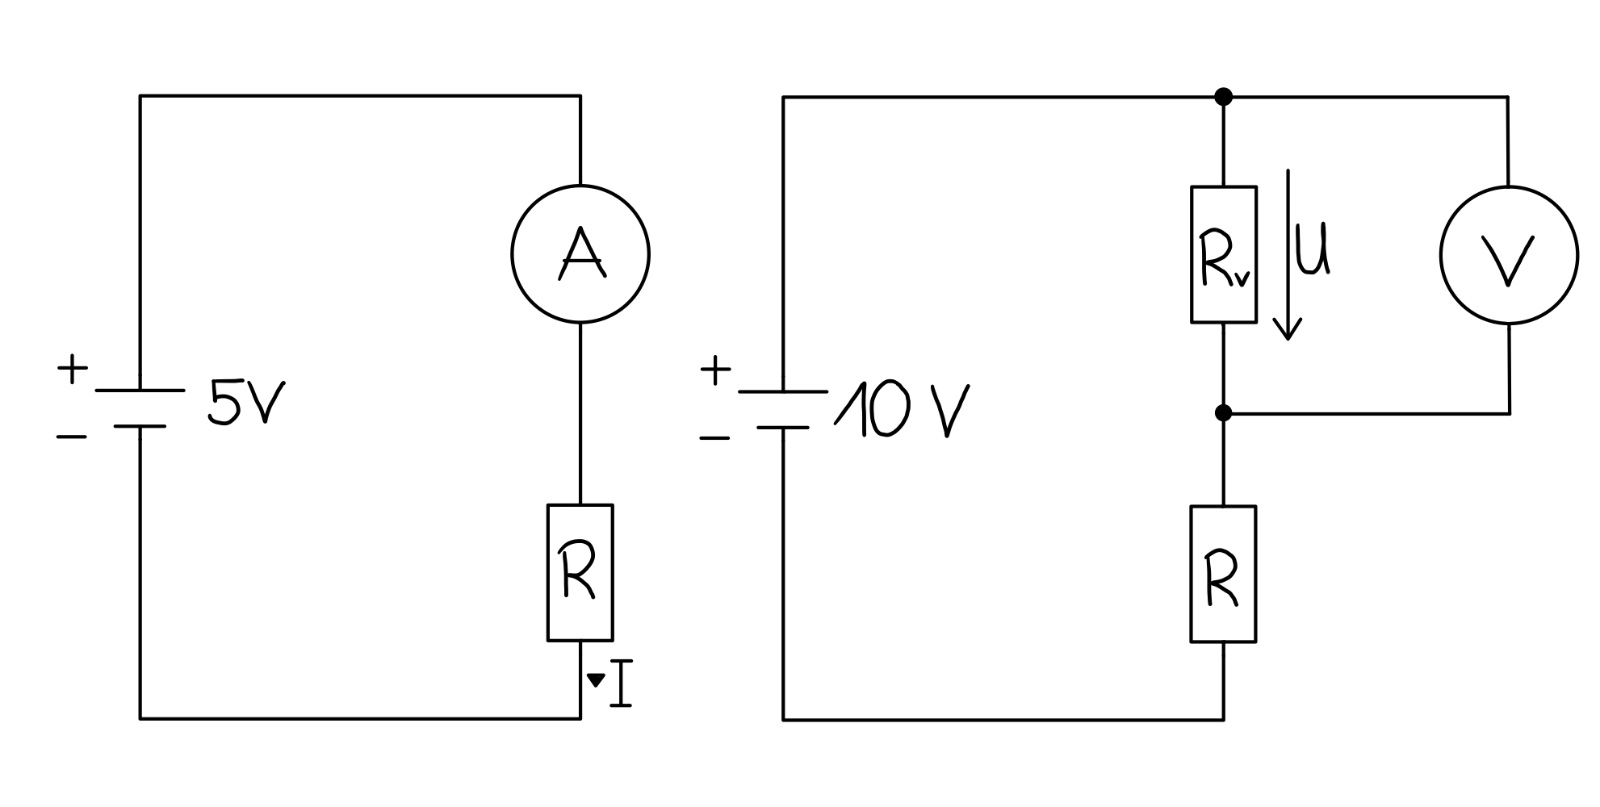
\includegraphics[width=0.7\textwidth]{../Quellen/Labor2/Schaltskizzen Widerstandsmessung.jpeg}
\caption{Schaltskizze 1 (Messung R) und Schaltskizze 2 (Messung R\textsubscript{V})}
\end{figure}



\begin{figure}[H]
    \centering
    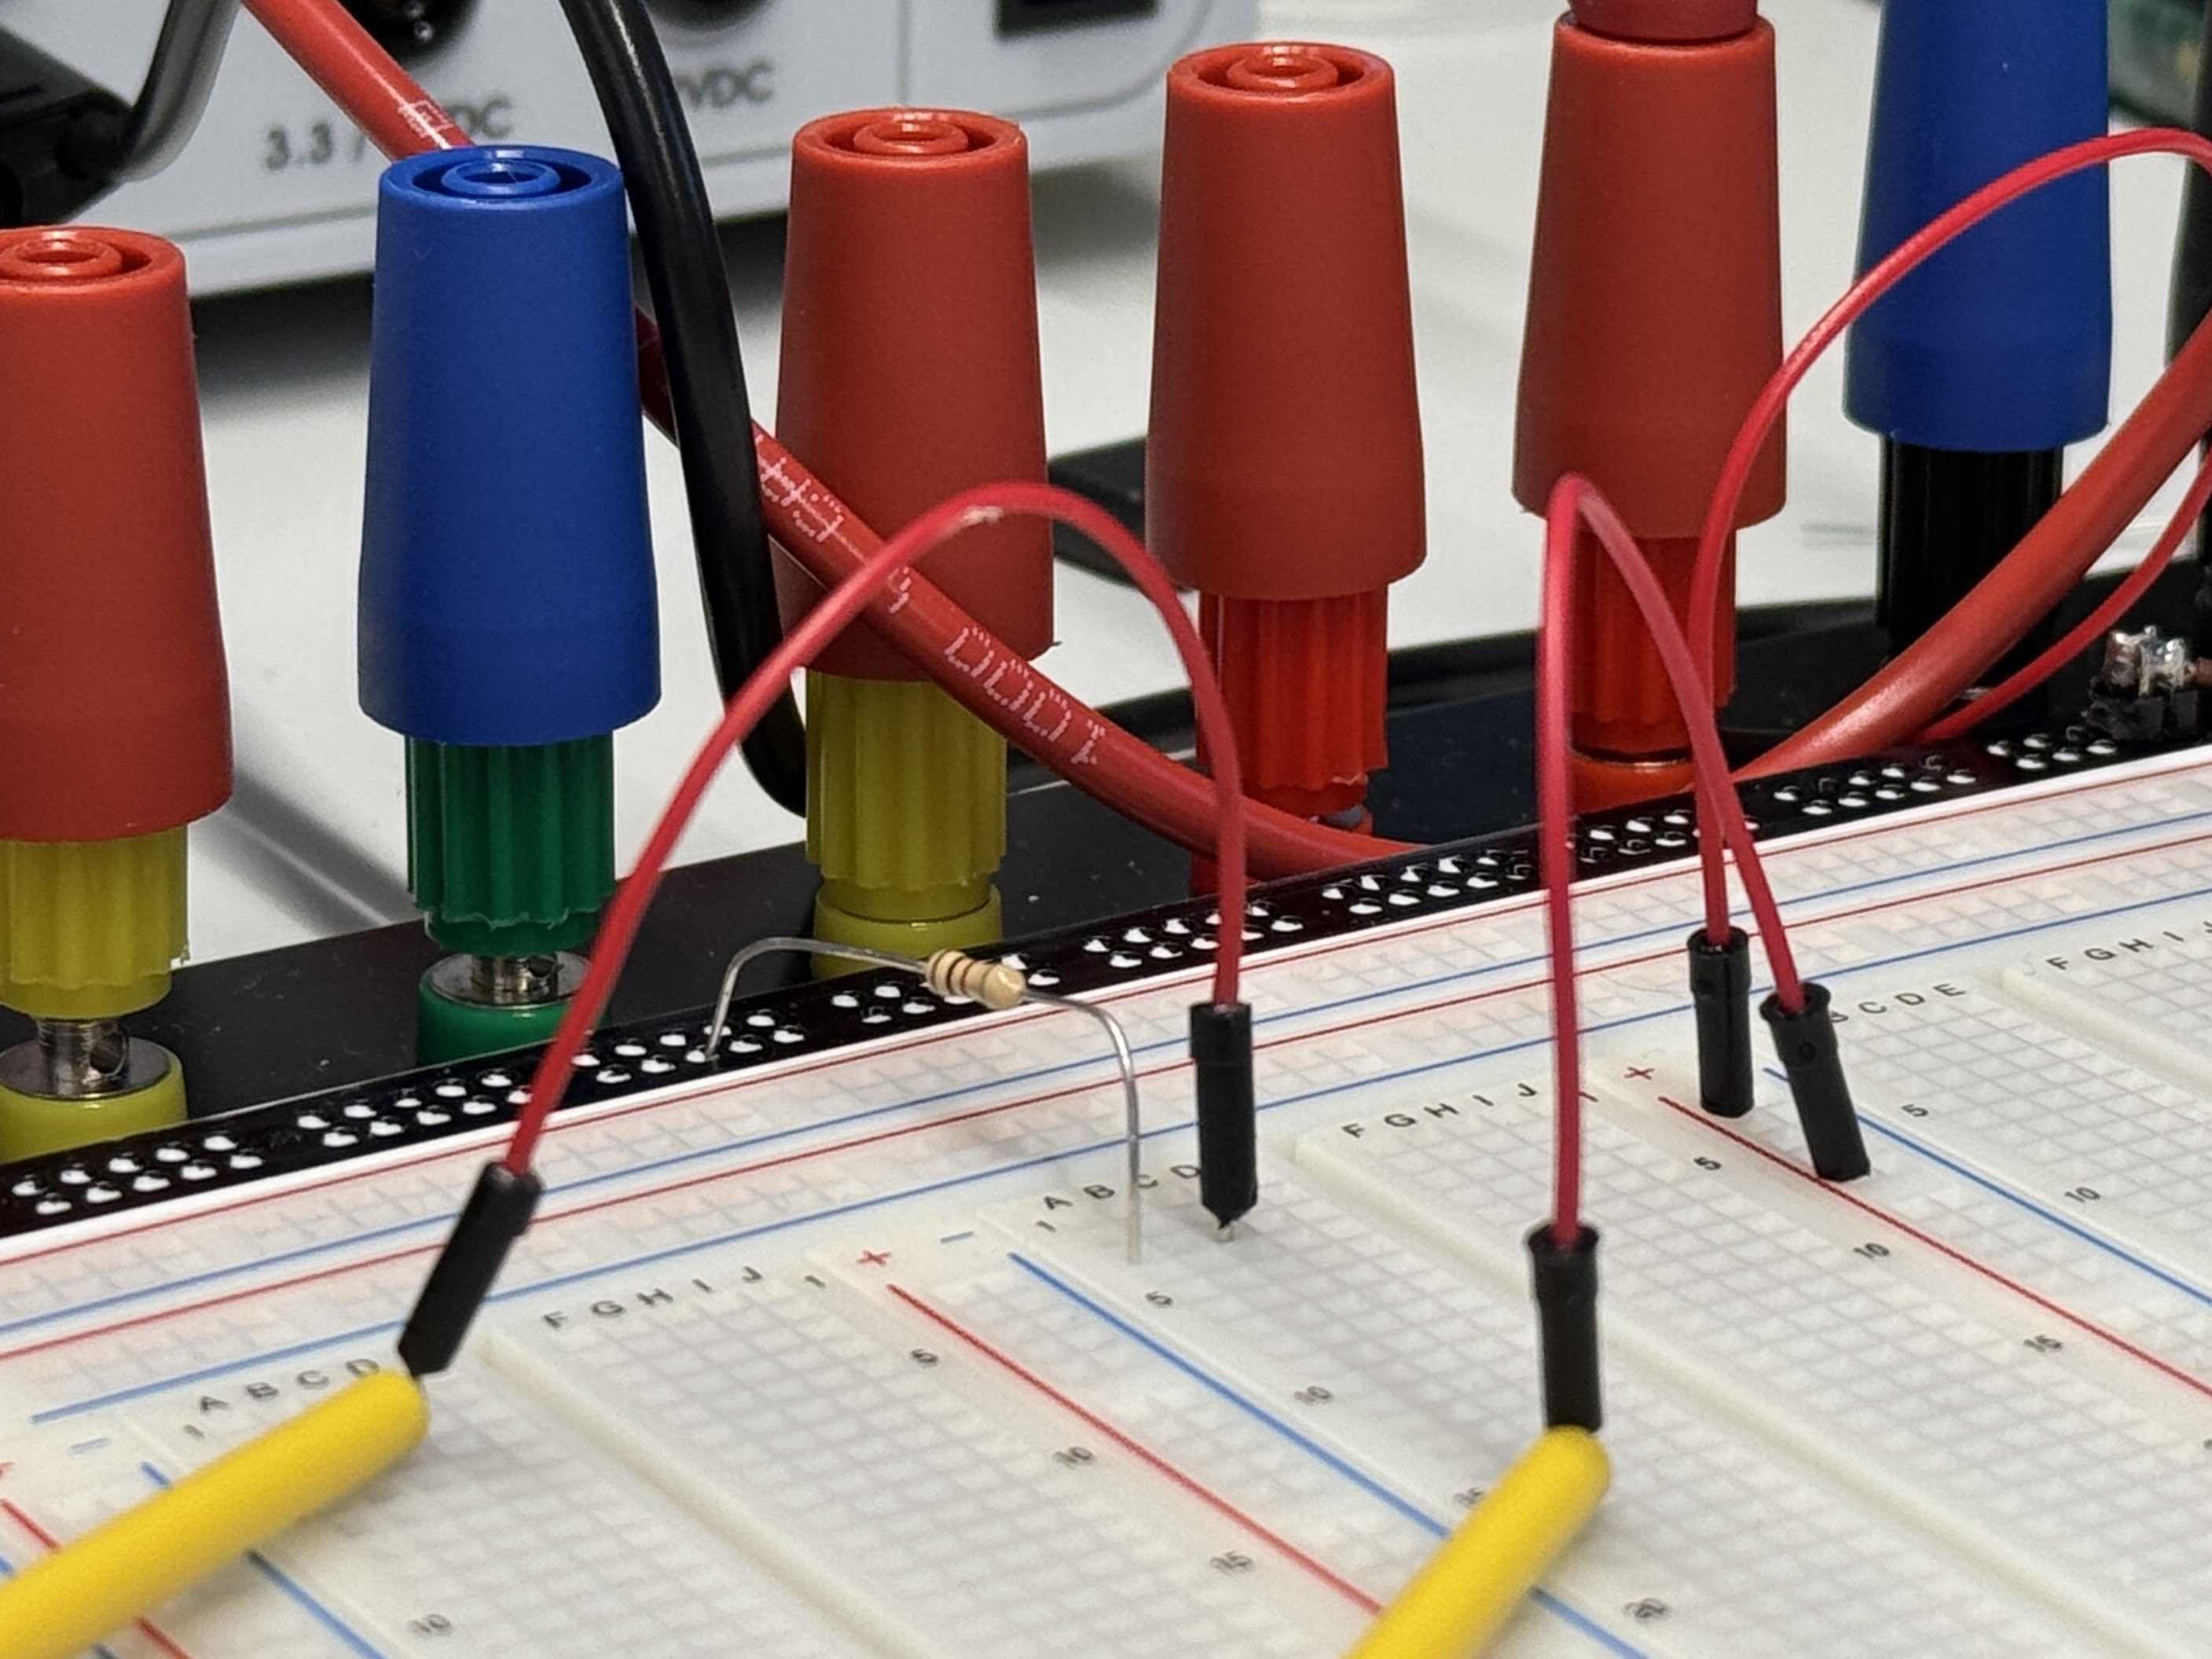
\includegraphics[width=0.65\textwidth]{../Quellen/Labor2/Fotos/IMG_3979.jpeg}
\caption{Messung R}
\end{figure}

\begin{figure}[H]
    \centering
    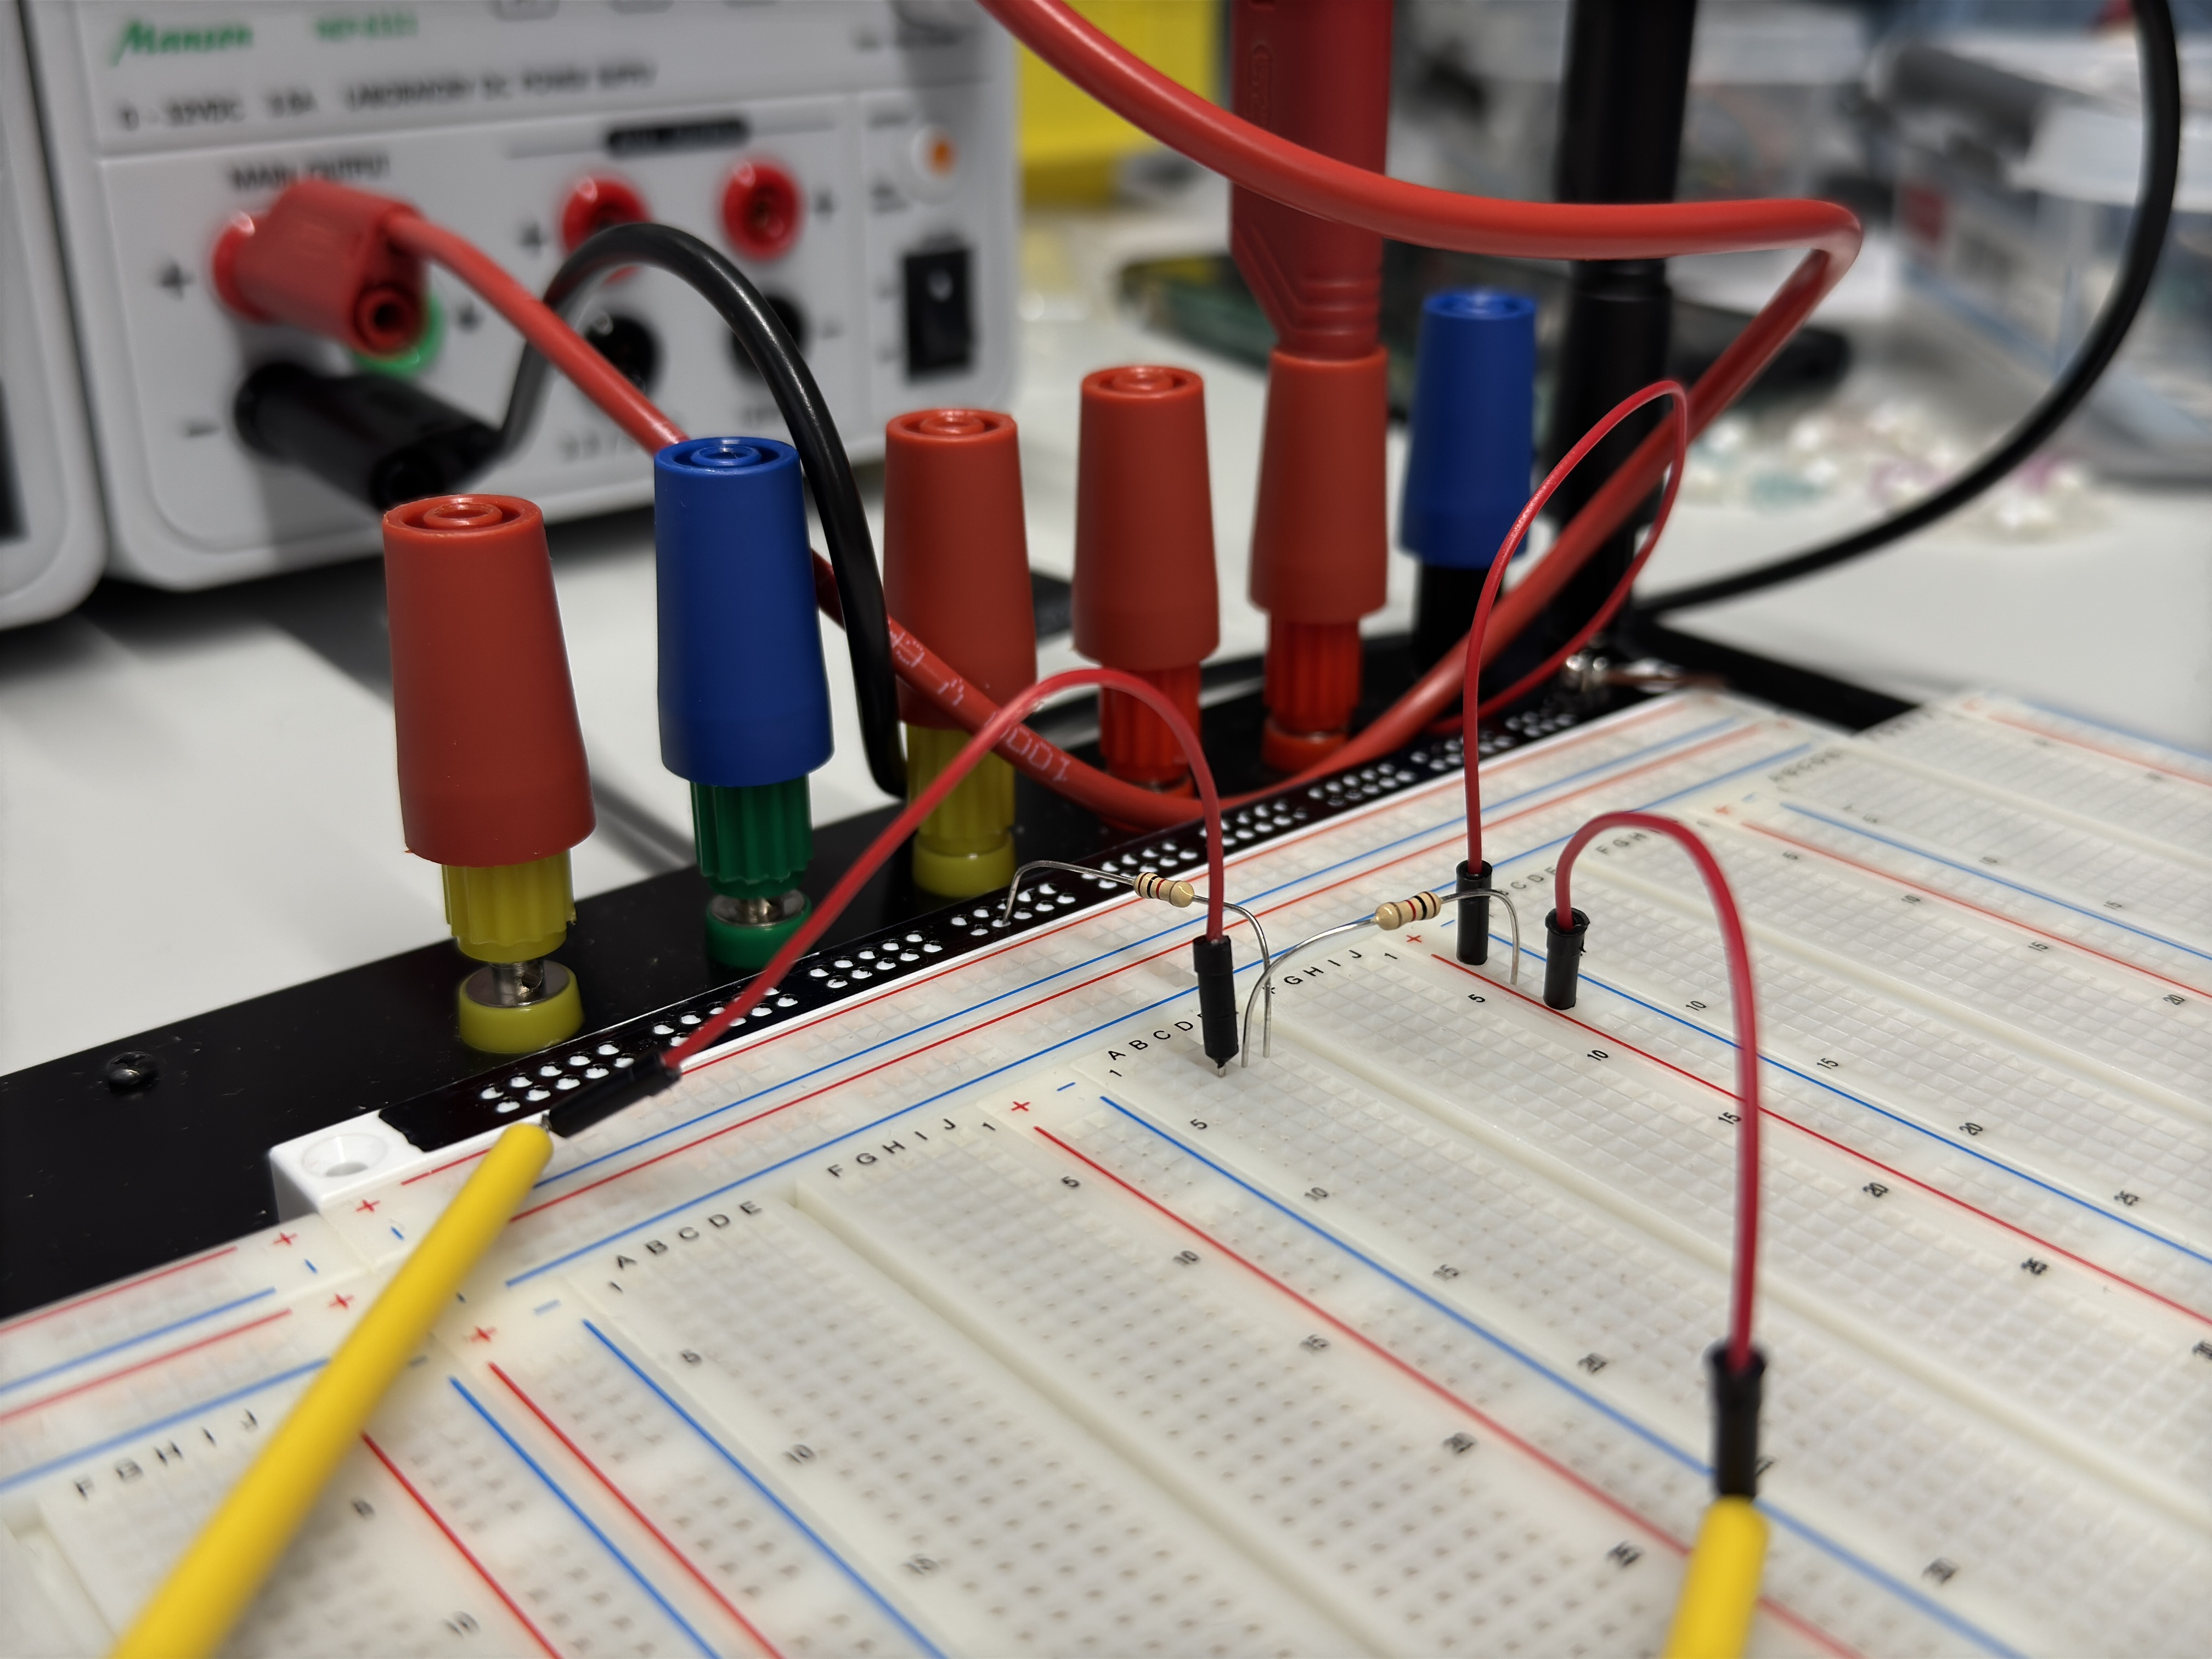
\includegraphics[width=0.65\textwidth]{../Quellen/Labor2/Fotos/IMG_3980.jpeg}
\caption{Messung R\textsubscript{V}}
\end{figure}


\subsection{Messergebnisse}
\begin{table}[H]
	\centering
	\begin{tabular}{|c|c|}
		\hline
		  & gemessener Widerstand in $\Omega$\\
		\hline		
		\textbf{R} & 988\\
		\hline
		\textbf{R\textsubscript{V}} & 996\\
		\hline
	\end{tabular}
	\caption{Nachmessung der Widerstände}
\end{table}
Begründen Sie aus den Betrachtungen der Fehlerrechnung, welches der beiden Verfahren b) oder c) 
eine genauere Bestimmung der Leistung ergibt.!!!!


\newpage
\section{Versuch 4: Widerstandsmessung mittels Vierdrahtmethode}
\subsection{Zielsetzung}
Es soll der (sehr niederohmige) Übergangswiderstand eines Kabels inklusive seiner Steckverbinder
mittels der Vierdrahtmethode gemessen werden. Der Fokus liegt darauf, möglichst Präzise den Widerstand des gesamten Kabels zu ermitteln, ohne die Werte mit der Messmethode zu verfälschen.

\subsection{Bauteile und Messgeräte}
\begin{itemize}
\item Labornetzgerät (NEP-8323)
\item Fluke 87 V True RMS Multimeter
\item Bananenkabel 2 Stück (Messobjekt und Messkabel)
\end{itemize}

\subsection{Messkonzept}
Das Messkonzept basiert auf der Nutzung der Vierdrahtmethode. Sie kann hohe Genauigkeit erzielen, was bei derart kleinen Widerständen, wie der eines Kabels, sehr von Vorteil ist. Im Detail wird der Messaufbau so realisiert, dass zwei separate Strom- und Spannungspfade verwendet werden. Dadurch, dass über die Messleitung kein Strom fließt, fällt dadurch dort nur sehr wenig Spannung ab und sie verfälscht so nicht den Widerstand.\\
\noindent Ein Multimeter hingegen würde den Messtrom über die Messleitung leiten und die dabei entstehenden Leitungswiderstände mitmessen. Diese parasitären Widerstände führen zu einer Verfälschung des Messergebnisses. \\\\
\noindent  {\bfseries Netzteil Einstellungen:\par}
\noindent Am Netzteil leuchtet die Anzeige für C.C (= Constant Current), was bedeutet, dass sich das Gerät im Konstantstrom Modus befindet und über Spannungsanpassungen den Strom konstant hält. Eine schlecht gewählt Einstellung der Strombegrenzung kann in diesem Modus verschiedene Effekte haben:
\begin{itemize}
\item Limit zu niedrig: Spannungsabfall zu klein, um vom Messgerät präzise gemssen zu werden. Höhere Ströme erzeugen einen größeren Spannungsabfall, der leichter und genauer zu messen ist, insbesondere bei niederohmigen Widerständen.
\item Limit zu hoch: Messtrom erwärmt das Objekt, wodurch der Widerstand steigt und das Ergebnis verfälscht wird.
\item Limit zu hoch: Überlastung des Netzerätes, Abschaltung\\
\end{itemize}
\newpage
\noindent  {\bfseries Die Grenzen der Strombegrenzung:\par}
\begin{itemize}
\item Seitens des Netzgeräts: Das Netzteil verfügt über eine maximale Stromausgabe von 3,5 A.
\item Seitens der Anwendung: Die genauen Spezifikationen des Kabels sind unbekannt. Typischerweise können Bananenkabel diesen Durchmessers mit etwa 30 A belastet werden. 
\item Bei anderen Anwendungen: 
	\begin{itemize}
	\item Bauteilschutz: In Anwendungen, die Halbleiterbauteilen oder andere empfindlichen Bauteile beinhalten, darf der Strom bestimmte Bauteilgrenzen nicht überschreiten, um Zerstörung oder Funktionsbeeinträchtigungen zu verhindern.
	\item Effizienz: Ein zu hoher Strom führt generell zu Energieverlusten.\\
	\end{itemize}
\end{itemize}
\noindent  {\bfseries Aufbau der Messschaltung:\par}
\noindent Um den gesamten Widerstand des Kabels inklusiver seiner Steckverbindungen, wie er bei reellen Nutzungssituationen vorkommt, zu ermitteln, muss die Reihenfolge der Steckverbindungen beachtet werden. 

\begin{figure}[H]
    \centering
    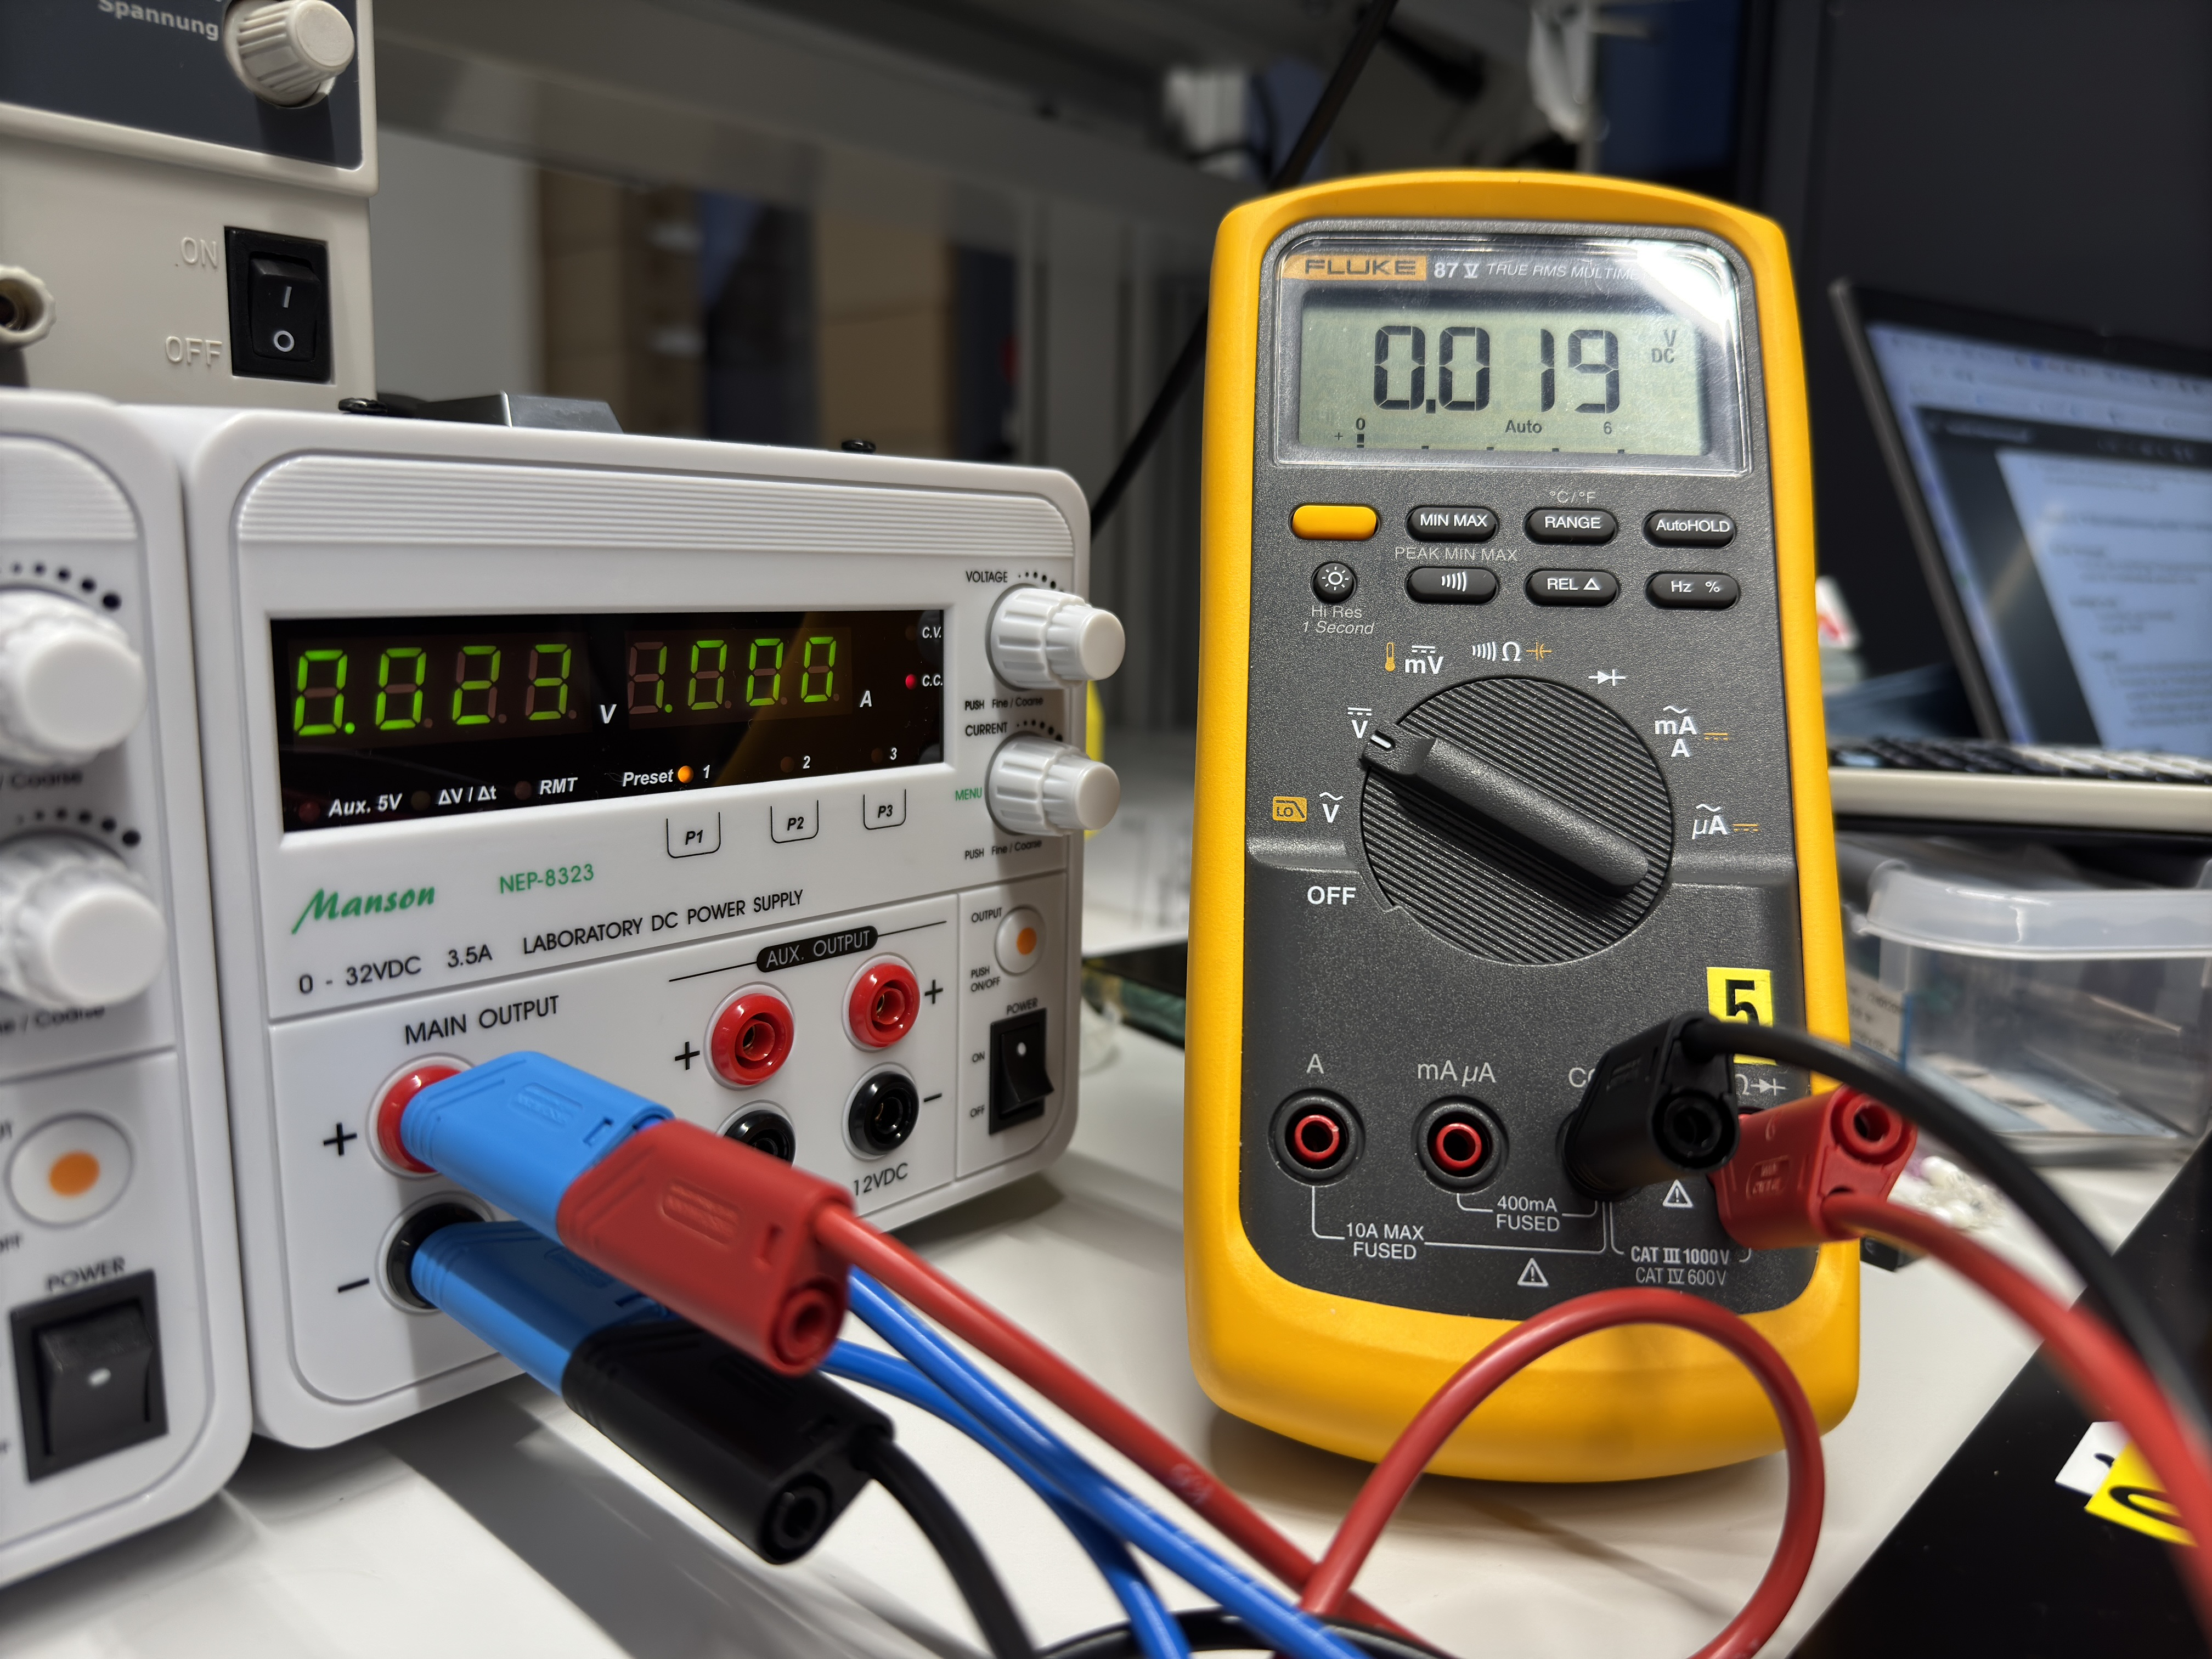
\includegraphics[width=0.7\textwidth]{../Quellen/Labor2/Fotos/IMG_3983.jpeg}
\caption{Teil der Steckverbindung nicht berücksichtigt}
\end{figure}

\begin{figure}[H]
    \centering
    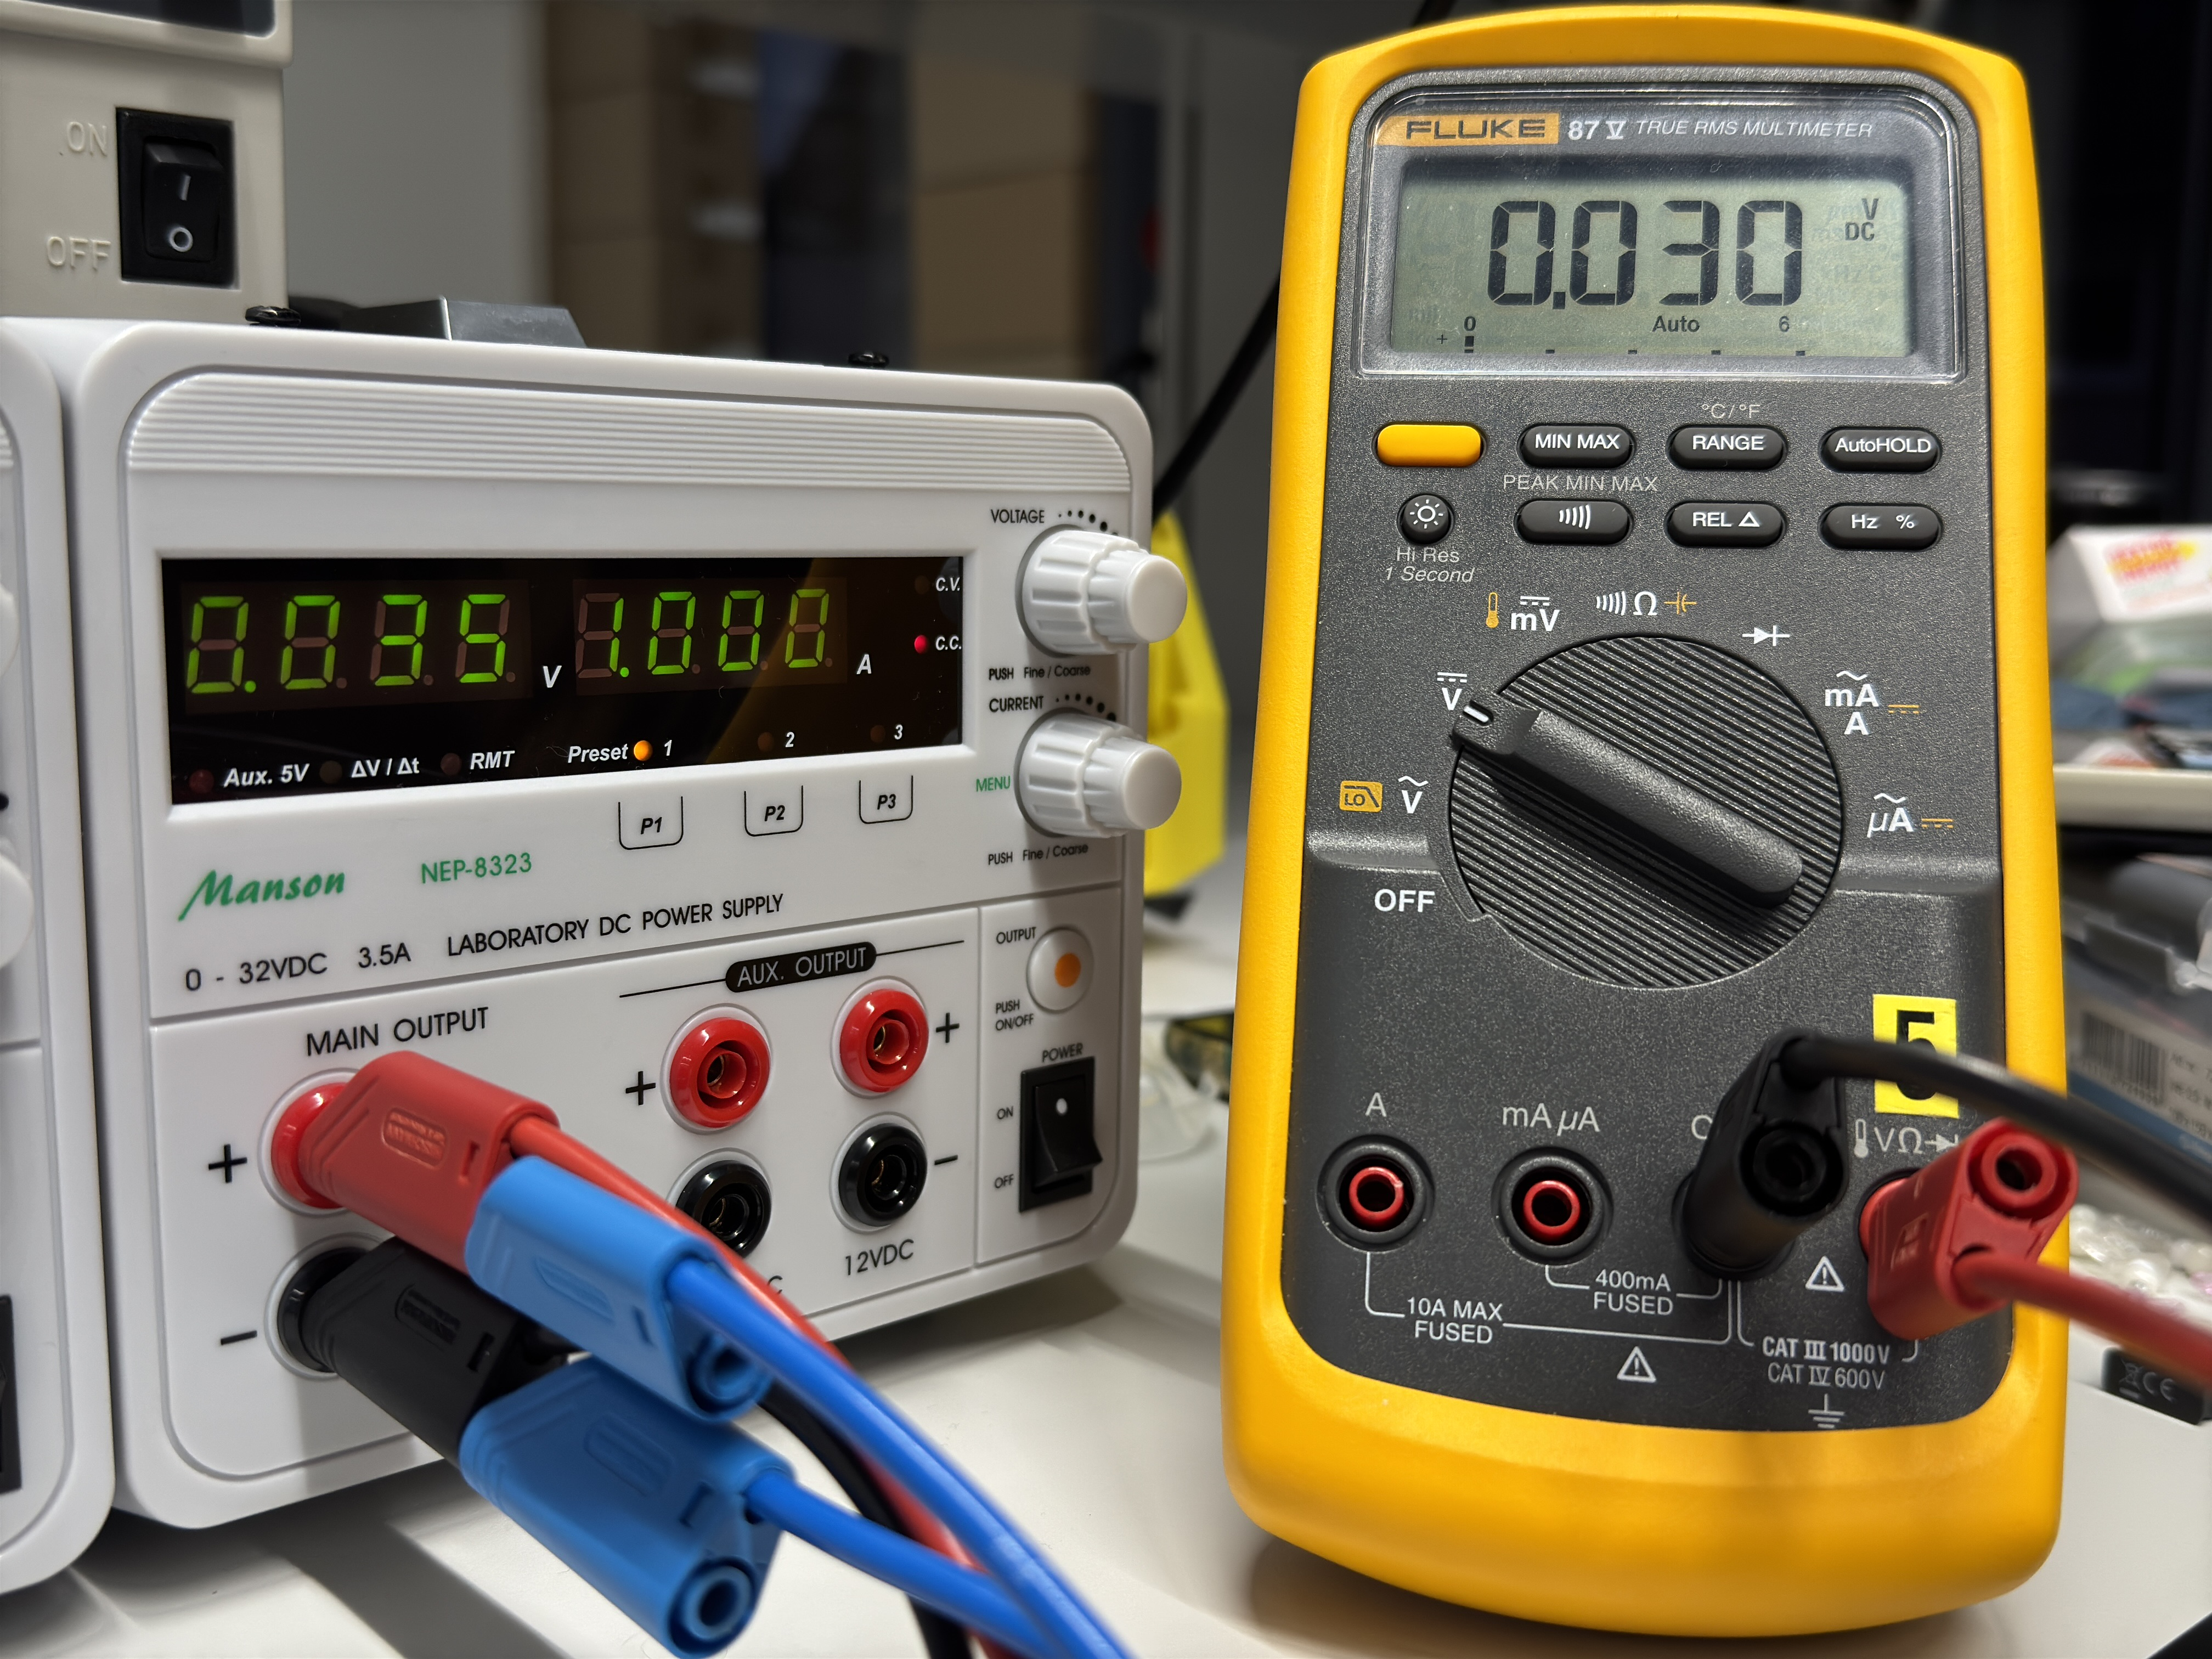
\includegraphics[width=0.7\textwidth]{../Quellen/Labor2/Fotos/IMG_3982.jpeg}
\caption{Messung über gesamtes Objekt inkl. der ganzen Steckverbindungen}
\end{figure}

\subsection{Messergebnisse}
Um den Widerstand des blauen Kabels zu berechnen, verwenden wir die Differenz der Spannungswerte zwischen dem Netzteil und dem Digitalmultimeter.\\\\
   - Spannung am Netzteil: \( U_{\text{Netzteil}} = 0,035 \, \text{V} \) \\
   - Spannung am DMM: \( U_{\text{DMM}} = 0,030 \, \text{V} \) \\
   - Strom durch das Kabel: \( I = 1,000 \, \text{A} \) \\\\
Spannungsabfall über das Kabel:
   \[
   \Delta U = U_{\text{Netzteil}} - U_{\text{DMM}} = 0,035 \, \text{V} - 0,030 \, \text{V} = 0,005 \, \text{V}
   \]\\
Berechnung des Widerstands:
   \[
   R = \frac{\Delta U}{I} = \frac{0,005 \, \text{V}}{1,000 \, \text{A}} = 0,005 \, \Omega
   \]

\newpage
\section{Versuch 5: Statistik}
\subsection{Zielsetzung}
Aufgabenstellung: Bestimmung einer gemessenen Zufallsverteilung und ihrer Eigenschaften (Momente). Hierbei stellt
das vorgegebene Los von Widerständen eine willkürlich entnommene Stichprobe einer vom
Hersteller erzeugten Grundgesamtheit dar.\\
\noindent Die Eigenschaften der gemessenen Zufallsverteilung zu bestimmen, insbesondere den Mittelwert und die empirische Standardabweichung. Diese Messung ermöglicht es, die Verteilung der Werte und die Toleranzen der Bauteile zu bewerten sowie zu untersuchen, inwieweit die gemessenen Ergebnisse mit den Herstellerangaben übereinstimmen.


\subsection{Bauteile und Messgeräte}
\begin{itemize}
\item Fluke 87 V True RMS Multimeter
\item Widerstandsgurt mit 25 Widerständen á 1,2 k$\Omega$
\end{itemize}

\subsection{Messkonzept}
Am Fluke Multimeter wird die Widerstandsmessung aktiviert. Es ermöglicht die Messung einzelner Widerstände mithilfe von Klemmen, die ans Multimeter angeschlossen werden. Mit dem Widerstand wird ein geschlossener Stromkreis gebildet, in dem das Multimeter den Widerstand mithilfe eines kleinen Messtroms bestimmt.\\
\noindent Bei dieser Messung können die parasitären Widerstände der Kabel vernachlässigt werden, da sie im Vergleich zu den zu messenden Widerstandsbauteilen verschwindend gering sind.

\begin{figure}[H]
    \centering
    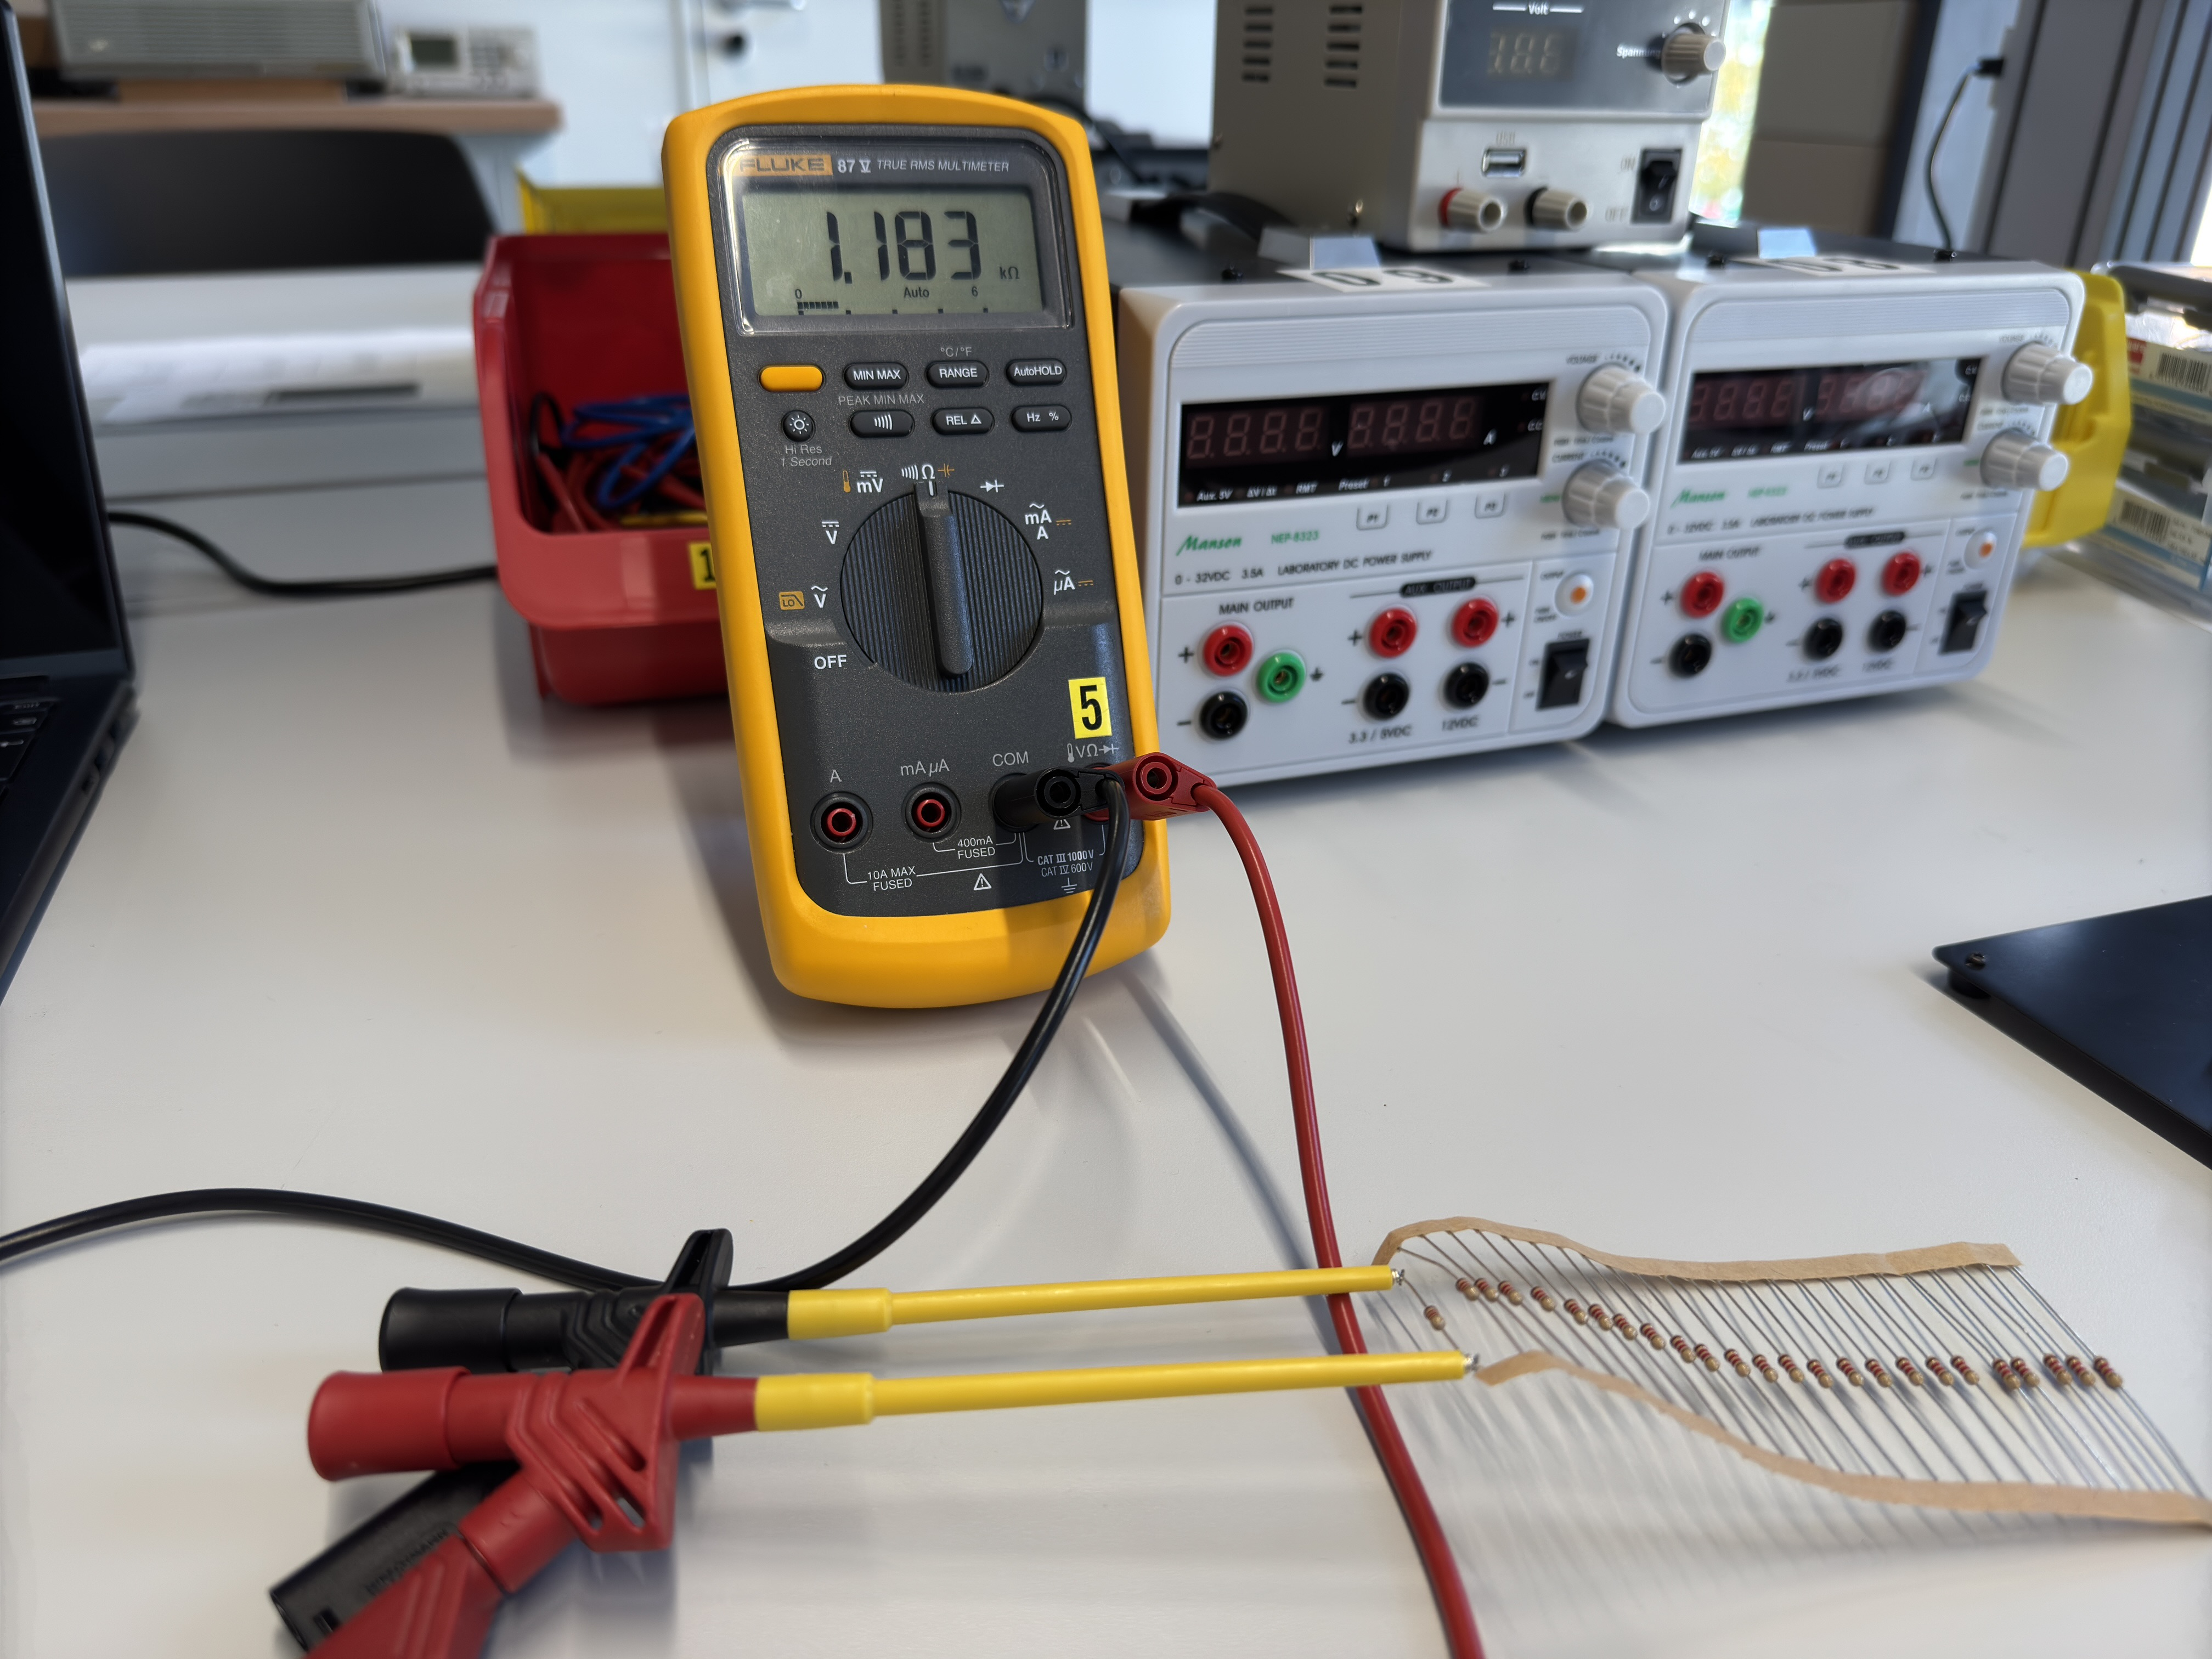
\includegraphics[width=0.7\textwidth]{../Quellen/Labor2/Fotos/IMG_4011.jpeg}
\caption{Messschaltung}
\end{figure}

\subsection{Messergebnisse}
\begin{table}[H]
	\centering
\scalebox{0.9}{	
	\begin{tabular}{|c|c|c|c|}
		\hline
		Widerstand Nr. & Wert in k$\Omega$ & Widerstand Nr. & Wert in k$\Omega$ \\
		\hline
		1 & 1.183 & 14 & 1.183 \\
		2 & 1.181 & 15 & 1.180 \\
		3 & 1.186 & 16 & 1.183 \\
		4 & 1.181 & 17 & 1.180 \\
		5 & 1.186 & 18 & 1.182 \\
		6 & 1.183 & 19 & 1.184 \\
		7 & 1.182 & 20 & 1.183 \\
		8 & 1.181 & 21 & 1.184 \\
		9 & 1.187 & 22 & 1.187 \\
		10 & 1.181 & 23 & 1.182 \\
		11 & 1.188 & 24 & 1.179 \\
		12 & 1.186 & 25 & 1.187 \\
		13 & 1.179 & - & - \\
		\hline
	\end{tabular}
}
	\caption{Einzelne Messungen}
\end{table}

\begin{figure}[H]
    \centering
    \includegraphics[width=0.7\textwidth]{../Quellen/Labor2/Histogramm-Widerstände.png}
\caption{Histogramm}
\end{figure}

\section*{Berechnung von Mittelwert und Standardabweichung}

Der Mittelwert \( \bar{x} \) wird berechnet als:
\[
\bar{x} = \frac{1}{n} \sum_{i=1}^{n} x_i = \frac{29.582}{25} = 1.1833 \, \text{k}\Omega
\]

Die empirische Standardabweichung \( s \) wird berechnet als:
\[
s = \sqrt{\frac{1}{n-1} \sum_{i=1}^{n} (x_i - \bar{x})^2}
\]

\textbf{Summe der quadratischen Abweichungen:}
\[
\sum_{i=1}^{n} (x_i - \bar{x})^2 = 0.000192
\]

\textbf{Einsetzen in die Formel:}
\[
s = \sqrt{\frac{0.000192}{25 - 1}} = \sqrt{0.000008} = 0.0028 \, \text{k}\Omega
\]

\begin{figure}[H]
    \centering
    \includegraphics[width=0.9\textwidth]{../Quellen/Labor2/Histogramm-Widerstände_Mittelwert_Std_Abweichung.png}
\caption{Histogramm mit Mittelwert und Standardabweichung}
\end{figure}

\noindent Zusätzlich zum Histogramm wurde die Kernel-Dichteschätzung (KDE) visualisiert, welche die Wahrscheinlichkeitsdichte darstellt. Im Gegensatz zum Histogramm, das die Verteilung durch diskrete Bins darstellt, erzeugt die KDE eine glatte, kontinuierliche Kurve.\\

\noindent Die Herstellertoleranz beträgt 5\% des Nominalwerts von \( 1.2 \, \text{k}\Omega \):
\[
\text{Toleranz} = \pm 0.05 \cdot 1.2 \, \text{k}\Omega = \pm 0.060 \, \text{k}\Omega
\]

\noindent Der Faktor zwischen der Toleranz und der empirischen Standardabweichung \( s \) wird berechnet als:
\[
\text{Faktor} = \frac{\text{Toleranz}}{s} = \frac{0.060 \, \text{k}\Omega}{0.00267 \, \text{k}\Omega} \approx 22.50
\]

\noindent Die großzügigen Toleranzen, wie sie von den Herstellern angegeben werden, helfen dabei, dass viele Bauteile innerhalb der spezifizierten Grenzen liegen. Eine großzügige Toleranz erhöht die Produktionsausbeute und senkt die Kosten.


\section*{Vergleich der invertierenden und nicht-invertierenden Grundschaltung eines Operationsverstärkers}

\subsection*{1. Allgemeine Spannungsverstärkung}
\textbf{Invertierende Schaltung:}~~~~~~\(A_V = -\frac{R_f}{R_{in}}\)

\noindent wobei:
\begin{itemize}
    \item \( R_f \) der Gegenkopplungswiderstand ist
    \item \( R_{in} \) der Eingangswiderstand ist
\end{itemize}

\noindent \textbf{Nicht-invertierende Schaltung:}~~~~~~\(A_V = 1 + \frac{R_f}{R_{in}}\)


\subsection*{2. Relative Verstärkungsänderung}
Angenommen, der Gegenkopplungswiderstand \( R_f \) wird durch einen Wert \( R_f + \Delta R_f \) ersetzt, wobei \( \Delta R_f \) die Abweichung aufgrund der Toleranz ist.
\subsubsection*{Invertierende Schaltung:}
\[
A_V' = -\frac{R_f + \Delta R_f}{R_{in}}
\]
Die relative Verstärkungsänderung \( \frac{\Delta A_V}{A_V} \) ist:
\[
\frac{\Delta A_V}{A_V} = \frac{A_V' - A_V}{A_V} = \frac{\left( -\frac{R_f + \Delta R_f}{R_{in}} \right) - \left( -\frac{R_f}{R_{in}} \right)}{-\frac{R_f}{R_{in}}}
\]
Vereinfachung:
\[
\frac{\Delta A_V}{A_V} = \frac{\Delta R_f}{R_f}
\]

\subsubsection*{Nicht-invertierende Schaltung:}
\[
A_V' = 1 + \frac{R_f + \Delta R_f}{R_{in}}
\]
Die relative Verstärkungsänderung \( \frac{\Delta A_V}{A_V} \) ist:
\[
\frac{\Delta A_V}{A_V} = \frac{A_V' - A_V}{A_V} = \frac{\left( 1 + \frac{R_f + \Delta R_f}{R_{in}} \right) - \left( 1 + \frac{R_f}{R_{in}} \right)}{1 + \frac{R_f}{R_{in}}}
\]
Vereinfachung:
\[
\frac{\Delta A_V}{A_V} = \frac{\frac{\Delta R_f}{R_{in}}}{1 + \frac{R_f}{R_{in}}}
\]

\subsection*{3. Empfindlichkeit der Schaltungen}
Die \textbf{invertierende Schaltung} ist proportional zur relativen Änderung \( \frac{\Delta R_f}{R_f} \), was bedeutet, dass die Verstärkungsänderung direkt von der Änderung des Gegenkopplungswiderstands abhängt.\\
\noindent Die \textbf{nicht-invertierende Schaltung} ist weniger empfindlich, da die Verstärkungsänderung durch den Faktor \( 1 + \frac{R_f}{R_{in}} \) abgeschwächt wird.\\
\noindent \textbf{Fazit:} Die invertierende Schaltung reagiert empfindlicher auf Änderungen des Gegenkopplungswiderstands.

\subsection*{4. Zahlenbeispiel}
Gegeben:
\[
 R_f = 10 \, \text{k}\Omega~~~~~~~~~~R_{in} = 1 \, \text{k}\Omega~~~~~~~~~~Toleranz~\Delta R_f = 5\%,~ also~\Delta R_f = 0,05 \times 10 \, \text{k}\Omega = 0,5 \, \text{k}\Omega
\]


\subsubsection*{Invertierende Schaltung:}
\[
\frac{\Delta A_V}{A_V} = \frac{\Delta R_f}{R_f} = \frac{0,5}{10} = 0,05 \quad \text{(5\% relative Änderung)}
\]

\subsubsection*{Nicht-invertierende Schaltung:}
\[
\frac{\Delta A_V}{A_V} = \frac{\frac{\Delta R_f}{R_{in}}}{1 + \frac{R_f}{R_{in}}} = \frac{\frac{0,5}{1}}{1 + \frac{10}{1}} = \frac{0,5}{11} \approx 0,0455 \quad \text{(4,55\% relative Änderung)}
\]

\noindent Die Resultate von Änderungen des Gegenkopplungswiderstands weisen auf, dass die nicht-invertierende Schaltung gegenüber der invertierende Schaltung um fast 10\% weniger empfindlich ist. 



\newpage
\section{Versuch 6: Aktiver Tiefpass erster Ordnung}
\subsection{Zielsetzung}

Die Zielsetzung des Versuches ist es, die frequenzabhängige Verstärkung eines aktiven Tiefpasses zu bestimmen. Dabei soll die Charakteristik des Filters analysiert und der Frequenzgang vermessen werden. Der Fokus liegt darauf, den Zusammenhang zwischen der Verstärkung und der Frequenz des Eingangssignals zu ermitteln und die Grenzfrequenz des Filters zu bestimmen.
\subsection{Bauteile und Messgeräte}
\begin{itemize}

\item Netzgerät (NEP-8323)
\item Fluke 87 V True RMS Multimeter
\item Keysight Oszilloskop (DSOX1102A)
\item Bananenkabel (mehrere: rot, blau, schwarz)
\item Oszilloskop BNC Tastkopf mit Messklemme
\item Steckkabel (mehrere: im Idealfall verschiedene Farben)
\item Steckbrett
\item Gegenkopplungs-Kondensator 10 µF "Tantalum"
\item Widerstände:
\[
 R_{1} = 1 \, \text{k}\Omega~~~~~~~R_{2} = 10 \, \text{k}\Omega~~~~~~~R = 1 \, \text{k}\Omega
\]
\end{itemize}
\subsection{Theorie hinter der Schaltung}
\begin{figure}[H]
    \centering
    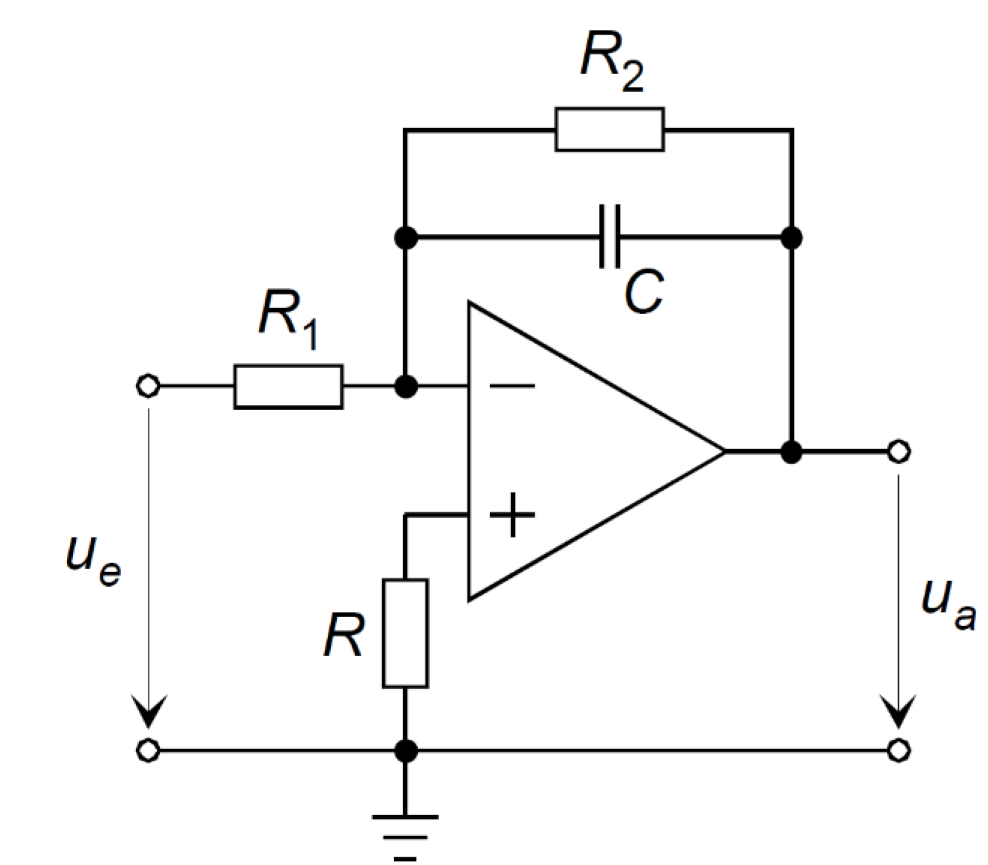
\includegraphics[width=0.5\textwidth]{../Quellen/Labor2/Versuch 6/Schaltungsplan.png}
\caption{Schaltskizze}
\end{figure}
In Figure 17 ist die Schaltskizze eines aktiven Tiefpasses zu sehen. Der Widerstand R stellt in dieser Schaltung sicher, dass ein definierter Gleichstrompfad für den Eingangsstrom des Operationsverstärkers vorhanden ist, sodass sich keine statische Ladung am nicht-invertierenden Eingang aufbauen kann. Ohne diesen Widerstand könnte es zu einer ungewollten Verschiebung des Arbeitspunktes kommen, was die Funktion der Schaltung beeinträchtigen würde. Eine weitere Aufgabe dieses Widerstandes ist es, Offset-Fehler zu reduzieren. Operationsverstärker weisen geringe Eingangsoffsetströme auf. Diese, durch Ströme verursachten, Spannungsunterschiede werden vom Widerstand R ausgeglichen, was die Genauigkeit der Schaltung verbessern kann.\\
Die Bemessung von R erfolgt in der Regel, dass sein Wert dem Wert des Ersatzwiderstands am invertierenden Eingang entspricht, also: \(
R \approx R_2 \parallel R_1\).\\
Dieser Wert stellt eine Balance her, sodass die Offsetspannung kompensiert wird, und trägt zu einer symmetrischen Belastung bei beiden Eingängen bei.\\
In der Wechselstromanalyse des Tiefpassfilters beeinflusst $R$ den Frequenzgang der Schaltung kaum, da er in der Regel sehr hoch im Vergleich zu den relevanten Impedanzen (z. B. dem Gegenkopplungsnetzwerk) dimensioniert ist. Da $R$ also nur den Gleichstrompfad definiert und keine wesentliche Rolle für die Signalverstärkung oder -dämpfung spielt, wird er in der Wechselstromanalyse der Schaltung meist vernachlässigt.

\noindent \textbf{Berechnung des Widerstandes R:}
\[
R = R_2 \parallel R_1 = \frac{R_2 \cdot R_1}{R_2 + R_1}~=~\frac{10 \, \text{k}\Omega \cdot 1 \, \text{k}\Omega}{10 \, \text{k}\Omega + 1 \, \text{k}\Omega} = \frac{10 \, \text{k}\Omega}{11} \approx 0{,}91 \, \text{k}\Omega
\]
In dieser Schaltung erfüllt der Kondensator $C$ die Funktion einer frequenzabhängigen Rückkopplung und bildet zusammen mit den Widerständen einen Tiefpassfilter in der Gegenkopplung des Operationsverstärkers.\\
\noindent Funktionsweise der Rückkopplung:
\begin{itemize}
\item Bei niedrigen Frequenzen: Der Kondensator hat einen hohen kapazitiven Widerstand (Impedanz), wodurch nur ein geringer Anteil des Signals rückgekoppelt wird. Die Verstärkung bleibt relativ hoch.
\item Bei höheren Frequenzen: Der kapazitive Widerstand des Kondensators nimmt ab, wodurch mehr Signal rückgekoppelt wird. Diese Rückkopplung reduziert die Verstärkung des Operationsverstärkers bei höheren Frequenzen, sodass der Ausgang des Tiefpassfilters das Signal nur für niedrige Frequenzen durchlässt und hohe Frequenzen dämpft.
\end{itemize}
\noindent Der Widerstand $R_2$ erfüllt eine wichtige Rolle in der \textbf{Bestimmung der Grenzfrequenz} und der \textbf{Einstellung der Verstärkung} des aktiven Tiefpasses.

\begin{itemize}
    \item \textbf{Bestimmung der Grenzfrequenz:} $R_2$ und $C$ bilden ein RC-Netzwerk, das die Grenzfrequenz des Filters definiert. Die Grenzfrequenz $f_c$ des Tiefpassfilters ergibt sich aus:
    \[
    f_c = \frac{1}{2 \pi R_2 C}
    \]
\end{itemize}





\subsection{Messkonzept}
Das Messkonzept basiert auf der Analyse der Schaltung eines aktiven Tiefpasses erster Ordnung, bestehend aus einem Operationsverstärker (OpAmp), Widerständen und einem Kondensator. Der Aufbau der Schaltung wird gemäß einer gegebenen Schaltskizze realisiert, und die Bauteile sind so dimensioniert, dass eine charakteristische Tiefpassfunktion entsteht.\\

\noindent \underline{Vorgehensweise:}\\
\noindent Die Schaltung wird auf einem Steckbrett (siehe Figure 18) aufgebaut, wobei der Operationsverstärker die Verstärkungs- und Filterfunktion übernimmt.
Ein Funktionsgenerator erzeugt Sinussignale mit unterschiedlichen Frequenzen, die als Eingangssignale an den Tiefpass angelegt werden.
Die Ausgangsspannung wird bei verschiedenen Frequenzen mit einem Oszilloskop gemessen, und die Verstärkung AV wird für jede Frequenz berechnet.
Der Frequenzbereich wird im 1:2:5-Muster durchlaufen, und im Bereich um die Grenzfrequenz wird die Frequenz besonders fein aufgelöst, um genaue Messdaten zu erhalten. Für diese Messreihe wurde als Signalform ein Sinussignal eingestellt. Die Messergebnisse sind in Table 5 aufgeführt.
Der gemessene Frequenzgang wird in einem doppelt-logarithmischen Diagramm dargestellt, um die Grenzfrequenz und die Charakteristik des Filters zu veranschaulichen.\\

\noindent \underline{Erwartungshaltung:}\\
\noindent Die Verstärkung sollte im niedrigen Frequenzbereich annähernd konstant sein und bei höheren Frequenzen abnehmen.
Die Grenzfrequenz fc, bei der die Verstärkung auf den Wert des Maximalwerts sinkt, wird ermittelt und im Diagramm dargestellt.

\begin{figure}[H]
    \centering
    \includegraphics[width=0.68\textwidth]{../Quellen/Labor2/Fotos/IMG_4023.jpeg}
\caption{Schaltungsaufbau}
\end{figure}
\noindent Die Funktion \(A\textsubscript{V}~=~\frac{u\textsubscript{a}}{u\textsubscript{e}}\) kann folgendermaßen als Funktion der Sinus-Signalfrequenz abgeleitet werden:
\[
Z\textsubscript{parallel}~=~\frac{1}{\frac{1}{Z\textsubscript{R\textsubscript{2}}}~+~\frac{1}{Z\textsubscript{C}}}~~~~~~~~~~Z\textsubscript{C}~=~\frac{1}{j\omega C}~~~~~~~~~~Z\textsubscript{R\textsubscript{2}}~=~R\textsubscript{2}
\]
\[
Z\textsubscript{parallel}~=~\frac{1}{\frac{1}{R\textsubscript{2}}~+~j\omega C}~=~\frac{R\textsubscript{2}}{1~+~j\omega CR\textsubscript{2}}
\]
\[
A\textsubscript{V}~=~\frac{u\textsubscript{a}}{u\textsubscript{e}}~=~-\frac{Z\textsubscript{parallel}}{R_1}~=~-\frac{R_2}{R_1}~\cdot~\frac{1}{1~+~j\omega CR\textsubscript{2}}
\]
\noindent Für den reellen Betrag von \(\left\lvert A\textsubscript{V}\right\rvert~=~\sqrt{A\textsubscript{V}~\cdot~(A\textsubscript{V})^*}\) gilt:
\[
\left\lvert A\textsubscript{V}\right\rvert~=~\sqrt{-\frac{R_2}{R_1}~\cdot~\frac{1}{1~+~j\omega CR\textsubscript{2}}~\cdot~-\frac{R_2}{R_1}~\cdot~\frac{1}{1~+~(-j)\omega CR\textsubscript{2}}}~=~\frac{R_2}{R_1}\cdot\frac{1}{\sqrt{1+(2\pi f\textsubscript{c} CR_2)^2}}
\]
\noindent Die Grenzfrequenz \(f\textsubscript{c}\) lässt sich durch \(f_c = \frac{1}{2 \pi R_2 C}\) berechnen.
\[
f\textsubscript{c}~=~\frac{1}{2 \pi~\cdot~10~k\Omega~\cdot~10~nF}~\approx~1.592~kHz
\]

\subsection{Messergebnisse}
\begin{table}[H]
	\centering
\scalebox{0.95}{	
	\begin{tabular}{|c|c|}
		\hline
		Frequenz f\textsubscript{c} in Hz & Amplitude in V \\
		\hline
		100 & 9.475 \\
		200 & 9.4 \\
		500 & 9.05 \\
		1000 & 7.975 \\
		2000 & 5.838 \\
		5000 & 2.894 \\
		10 000 & 1.545 \\
		20 000 & 0.825 \\
		50 000 & 0.338 \\
		100 000 & 0.241 \\
		\hline
	\end{tabular}
}
	\caption{Frequenzgang des aktiven Tiefpasses}
\end{table}
Bei einer Frequenz von 16 100 Hz bzw. beim Übereinanderlegen der Signale bei 17 300~Hz erreicht die Verstärkung den Wert 1. Diese Frequenz wird Transitfrequenz genannt.


























\section{Diskussion}
Was würden Sie nächstes Mal anders machen? Was hat besondere Schwierigkeiten bereitet?\\

- Nr. 3 eine Frage in rot\\
-Versuch 6 c) fertigmachen, d),e)g)


\end{document}
